%% LyX 2.0.5.1 created this file.  For more info, see http://www.lyx.org/.
%% Do not edit unless you really know what you are doing.
\documentclass[11pt,english]{yalephd}
\usepackage[T1]{fontenc}
\usepackage[latin9]{inputenc}
\usepackage{geometry}
\geometry{verbose,tmargin=1in,bmargin=1in,lmargin=1.5in,rmargin=1in}
\setcounter{secnumdepth}{3}
\setcounter{tocdepth}{3}
\usepackage{color}
\usepackage{float}
\usepackage{graphicx}

\makeatletter

%%%%%%%%%%%%%%%%%%%%%%%%%%%%%% LyX specific LaTeX commands.
%% Because html converters don't know tabularnewline
\providecommand{\tabularnewline}{\\}
%% A simple dot to overcome graphicx limitations
\newcommand{\lyxdot}{.}


%%%%%%%%%%%%%%%%%%%%%%%%%%%%%% User specified LaTeX commands.



\usepackage{geometry} % you need this for yalephd.cls to work.
\usepackage{graphicx} % you probably want the rest of these.
\usepackage{dcolumn}
\usepackage{bm}
\usepackage{amsmath}
\usepackage{amsfonts}
\usepackage{amssymb}
\usepackage{appendix}
\usepackage{comment}
\usepackage{cite}
\usepackage{notoccite}


\newcommand{\mvir}{M_{\rm vir}}
\newcommand{\mcoll}{M_{\rm coll}}
\newcommand{\rvir}{R_{\rm vir}}
\newcommand{\vmax}{V_{\rm max}}
\newcommand{\meanvmax}{\overline{V}_{\rm max}}

\newcommand{\ximm}{\xi_{\rm mm}}
\newcommand{\xihm}{\xi_{\rm hm}}
\newcommand{\bh}{b_{\rm h}}
\newcommand{\bhlin}{b^{\rm lin}_{\rm h}}

%%% UNITS %%%
\newcommand{\msun}{M_{\odot}/h}
\newcommand{\mpch}{{\rm Mpc}/h}
\newcommand{\kpch}{{\rm kpc}/h}


%-------------
\let\jnl@style=\rmfamily
\def\ref@jnl#1{{\jnl@style#1}}%
\newcommand\aj{\ref@jnl{AJ}}%
          % Astronomical Journal
\newcommand\actaa{\ref@jnl{Acta Astron.}}%
  % Acta Astronomica
\newcommand\araa{\ref@jnl{ARA\&A}}%
          % Annual Review of Astron and Astrophys
\newcommand\apj{\ref@jnl{ApJ}}%
          % Astrophysical Journal
\newcommand\apjl{\ref@jnl{ApJ}}%
          % Astrophysical Journal, Letters
\newcommand\apjs{\ref@jnl{ApJS}}%
          % Astrophysical Journal, Supplement
\newcommand\ao{\ref@jnl{Appl.~Opt.}}%
          % Applied Optics
\newcommand\apss{\ref@jnl{Ap\&SS}}%
          % Astrophysics and Space Science
\newcommand\aap{\ref@jnl{A\&A}}%
          % Astronomy and Astrophysics
\newcommand\aapr{\ref@jnl{A\&A~Rev.}}%
          % Astronomy and Astrophysics Reviews
\newcommand\aaps{\ref@jnl{A\&AS}}%
          % Astronomy and Astrophysics, Supplement
\newcommand\azh{\ref@jnl{AZh}}%
          % Astronomicheskii Zhurnal
\newcommand\baas{\ref@jnl{BAAS}}%
          % Bulletin of the AAS
\newcommand\caa{\ref@jnl{Chinese Astron. Astrophys.}}%
  % Chinese Astronomy and Astrophysics
\newcommand\cjaa{\ref@jnl{Chinese J. Astron. Astrophys.}}%
  % Chinese Journal of Astronomy and Astrophysics
\newcommand\icarus{\ref@jnl{Icarus}}%
  % Icarus
\newcommand\jcap{\ref@jnl{J. Cosmology Astropart. Phys.}}%
  % Journal of Cosmology and Astroparticle Physics
\newcommand\jrasc{\ref@jnl{JRASC}}%
          % Journal of the RAS of Canada
\newcommand\memras{\ref@jnl{MmRAS}}%
          % Memoirs of the RAS
\newcommand\mnras{\ref@jnl{MNRAS}}%
          % Monthly Notices of the RAS
\newcommand\na{\ref@jnl{New A}}%
  % New Astronomy
\newcommand\nar{\ref@jnl{New A Rev.}}%
  % New Astronomy Review
\newcommand\pra{\ref@jnl{Phys.~Rev.~A}}%
          % Physical Review A: General Physics
\newcommand\prb{\ref@jnl{Phys.~Rev.~B}}%
          % Physical Review B: Solid State
\newcommand\prc{\ref@jnl{Phys.~Rev.~C}}%
          % Physical Review C
\newcommand\prd{\ref@jnl{Phys.~Rev.~D}}%
          % Physical Review D
\newcommand\pre{\ref@jnl{Phys.~Rev.~E}}%
          % Physical Review E
\newcommand\prl{\ref@jnl{Phys.~Rev.~Lett.}}%
          % Physical Review Letters
\newcommand\pasa{\ref@jnl{PASA}}%
  % Publications of the Astron. Soc. of Australia
\newcommand\pasp{\ref@jnl{PASP}}%
          % Publications of the ASP
\newcommand\pasj{\ref@jnl{PASJ}}%
          % Publications of the ASJ
\newcommand\qjras{\ref@jnl{QJRAS}}%
          % Quarterly Journal of the RAS
\newcommand\rmxaa{\ref@jnl{Rev. Mexicana Astron. Astrofis.}}%
  % Revista Mexicana de Astronomia y Astrofisica
\newcommand\skytel{\ref@jnl{S\&T}}%
          % Sky and Telescope
\newcommand\solphys{\ref@jnl{Sol.~Phys.}}%
          % Solar Physics
\newcommand\sovast{\ref@jnl{Soviet~Ast.}}%
          % Soviet Astronomy
\newcommand\ssr{\ref@jnl{Space~Sci.~Rev.}}%
          % Space Science Reviews
\newcommand\zap{\ref@jnl{ZAp}}%
          % Zeitschrift fuer Astrophysik
\newcommand\nat{\ref@jnl{Nature}}%
          % Nature
\newcommand\iaucirc{\ref@jnl{IAU~Circ.}}%
          % IAU Cirulars
\newcommand\aplett{\ref@jnl{Astrophys.~Lett.}}%
          % Astrophysics Letters and Communications
\newcommand\apspr{\ref@jnl{Astrophys.~Space~Phys.~Res.}}%
          % Astrophysics Space Physics Research
\newcommand\bain{\ref@jnl{Bull.~Astron.~Inst.~Netherlands}}%
          % Bulletin Astronomical Institute of the Netherlands
\newcommand\fcp{\ref@jnl{Fund.~Cosmic~Phys.}}%
          % Fundamental Cosmic Physics
\newcommand\gca{\ref@jnl{Geochim.~Cosmochim.~Acta}}%
          % Geochimica Cosmochimica Acta
\newcommand\grl{\ref@jnl{Geophys.~Res.~Lett.}}%
          % Geophysics Research Letters
\newcommand\jcp{\ref@jnl{J.~Chem.~Phys.}}%
          % Journal of Chemical Physics
\newcommand\jgr{\ref@jnl{J.~Geophys.~Res.}}%
          % Journal of Geophysical Research
\newcommand\jqsrt{\ref@jnl{J.~Quant.~Spec.~Radiat.~Transf.}}%
          % Journal of Quantitiative Spectroscopy and Radiative Trasfer
\newcommand\memsai{\ref@jnl{Mem.~Soc.~Astron.~Italiana}}%
          % Mem. Societa Astronomica Italiana
\newcommand\nphysa{\ref@jnl{Nucl.~Phys.~A}}%
          % Nuclear Physics A
\newcommand\physrep{\ref@jnl{Phys.~Rep.}}%
          % Physics Reports
\newcommand\physscr{\ref@jnl{Phys.~Scr}}%
          % Physica Scripta
\newcommand\planss{\ref@jnl{Planet.~Space~Sci.}}%
          % Planetary Space Science
\newcommand\procspie{\ref@jnl{Proc.~SPIE}}%
          % Proceedings of the SPIE
\let\astap=\aap
\let\apjlett=\apjl
\let\apjsupp=\apjs
\let\applopt=\ao
\newcommand\phn{\phantom{0}}%
\newcommand\phd{\phantom{.}}%
\newcommand\phs{\phantom{$-$}}%
\newcommand\phm[1]{\phantom{#1}}%
\let\la=\lesssim            % For Springer A&A compliance...
\let\ga=\gtrsim
\newcommand\sq{\mbox{\rlap{$\sqcap$}$\sqcup$}}%
\newcommand\arcdeg{\mbox{$^\circ$}}%
\newcommand\arcmin{\mbox{$^\prime$}}%
\newcommand\arcsec{\mbox{$^{\prime\prime}$}}%
\newcommand\fd{\mbox{$.\!\!^{\mathrm d}$}}%
\newcommand\fh{\mbox{$.\!\!^{\mathrm h}$}}%
\newcommand\fm{\mbox{$.\!\!^{\mathrm m}$}}%
\newcommand\fs{\mbox{$.\!\!^{\mathrm s}$}}%
\newcommand\fdg{\mbox{$.\!\!^\circ$}}%
\newcommand\farcm@mss{\mbox{$.\mkern-4mu^\prime$}}%
\let\farcm\farcm@mss
\newcommand\farcs@mss{\mbox{$.\!\!^{\prime\prime}$}}%
\let\farcs\farcs@mss
\newcommand\fp{\mbox{$.\!\!^{\scriptscriptstyle\mathrm p}$}}%
\newcommand\micron{\mbox{$\mu$m}}%
\def\farcm@apj{%
 \mbox{.\kern -0.7ex\raisebox{.9ex}{\scriptsize$\prime$}}%
}%
\def\farcs@apj{%
 \mbox{%
  \kern  0.13ex.%
  \kern -0.95ex\raisebox{.9ex}{\scriptsize$\prime\prime$}%
  \kern -0.1ex%
 }%
}%
\newcommand\case[2]{\mbox{$\frac{#1}{#2}$}}%
\newcommand\slantfrac{\case}%
\newcommand\onehalf{\slantfrac{1}{2}}%
\newcommand\onethird{\slantfrac{1}{3}}%
\newcommand\twothirds{\slantfrac{2}{3}}%
\newcommand\onequarter{\slantfrac{1}{4}}%
\newcommand\threequarters{\slantfrac{3}{4}}%
\newcommand\ubvr{\mbox{$U\!BV\!R$}}%% UBVR system
\newcommand\ub{\mbox{$U\!-\!B$}}%   % U-B
\newcommand\bv{\mbox{$B\!-\!V$}}%   % B-V
\newcommand\vr{\mbox{$V\!-\!R$}}%   % V-R
\newcommand\ur{\mbox{$U\!-\!R$}}%   % U-R
\newcommand\ion[2]{#1$\;${\small\rmfamily\@Roman{#2}}\relax}%
\newcommand\nodata{ ~$\cdots$~ }%
\newcommand\diameter{\ooalign{\hfil/\hfil\crcr\mathhexbox20D}}%
\newcommand\degr{\arcdeg}%
\newcommand\Sun{\sun}% Sun symbol, "S"
\newcommand\Sol{\sun}%
\newcommand\sun{\odot}%
\newcommand\Mercury{\astro{\char1}}% Mercury symbol, "1"
\newcommand\Venus{\astro{\char2}}% Venus symbol, "2"
\newcommand\Earth{\earth}% Earth symbol, "3"
\newcommand\Terra{\earth}%
\newcommand\earth{\oplus}%
\newcommand\Mars{\astro{\char4}}% Mars symbol, "4"
\newcommand\Jupiter{\astro{\char5}}% Jupiter symbol, "5"
\newcommand\Saturn{\astro{\char6}}% Saturn symbol, "6"
\newcommand\Uranus{\astro{\char7}}% Uranus symbol, "7"
\newcommand\Neptune{\astro{\char8}}% Neptune symbol, "8"
\newcommand\Pluto{\astro{\char9}}% Pluo symbol, "9"
\newcommand\Moon{\astro{\char10}}% Moon symbol, "M"
\newcommand\Luna{\Moon}%
\newcommand\Aries{\astro{\char11}}%
\newcommand\VEq{\Aries}% vernal equinox (Aries)
\newcommand\Taurus{\astro{\char12}}%
\newcommand\Gemini{\astro{\char13}}%
\newcommand\Cancer{\astro{\char14}}%
\newcommand\Leo{\astro{\char15}}%
\newcommand\Virgo{\astro{\char16}}%
\newcommand\Libra{\astro{\char17}}%
\newcommand\AEq{\Libra}% autumnal equinox (Libra)
\newcommand\Scorpius{\astro{\char18}}%
\newcommand\Sagittarius{\astro{\char19}}%
\newcommand\Capricornus{\astro{\char20}}%
\newcommand\Aquarius{\astro{\char21}}%
\newcommand\Pisces{\astro{\char22}}%

\makeatother

\usepackage{babel}
\begin{document}

\section{Introduction}

Baryon acoustic oscillations are a signature of the early Universe
imprinted in the distribution of galaxies and dark matter (DM) at
the present epoch. As the early Universe expands and its temperature
drops, sound waves propagating in the baryon-photon plasma freeze
into the matter distribution at decoupling. This leaves a characteristic
peak in two-point correlation functions where the position of the
peak is $\sim150{\rm Mpc}$. The BAO method utilizes this characteristic
scale of the sound horizon as a standard ruler (e.g., \cite{1997PhRvL..79.3806T,1998ApJ...495...29G,1999MNRAS.304...75E}).

While the primordial density fluctuations are linear and well understood,
distribution of galaxies, which are biased tracers of the DM particles,
suffers from non-linear growth of structure, redshift-space distortions,
and galaxy biases. All these effects shift and broaden the BAO peak,
which causes a systematic bias and increases errors on distance measurements.
Many studies addressed how to quantify these effects analytically
(e.g., \cite{2009PhRvD..80f3508P}) and numerically (e.g., \cite{2008ApJ...686...13S,2010ApJ...720.1650S,2011ApJ...734...94M}).
Ref. \cite{2009PhRvD..80f3508P} show that the shift on the acoustic
scale is expected to be less than one percent, even with a presence
of galaxy bias using perturbation theory. For the case of DM, Ref.
\cite{2010ApJ...720.1650S} confirmed that the shift due to non-linear
evolution of structure and redshift-space distortions is about $0.3\pm0.015\%$
at $z=0.3$. Ref. \cite{2011ApJ...734...94M} showed a large but less
than one percent shift for the case of galaxies.

\textcolor{black}{In order to reduce the systematic errors on the
measurements, Ref. \cite{eisenstein2007} proposed a method termed
\textquotedblleft{}reconstruction\textquotedblright{} to account for
the effects of the non-linear evolution on large scales. This method
suppresses the non-linearities in the density field and sharpens the
BAO peak, as schematically shown in Fig. \ref{fig:bao_recon1}. Padmanabhan
et al. showed how the reconstruction method can sharpen the BAO peak
using perturbation theory. Furthermore, this technique has been widely
used in observational studies and successfully reduce the errors to
$\sim1\%$ }(e.g., \cite{2016arXiv160703155A})\textcolor{black}{.}

\begin{figure}[t]
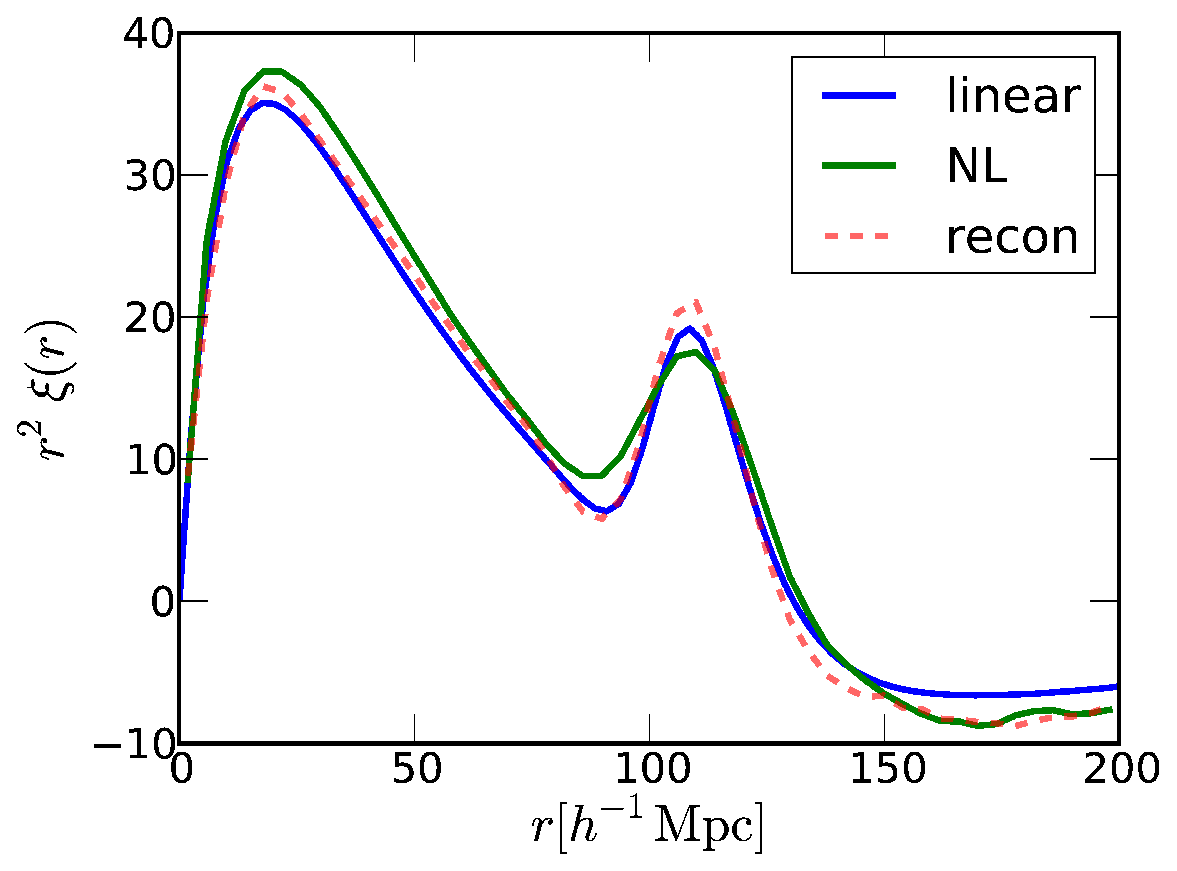
\includegraphics[width=0.5\textwidth]{/Users/old_ts485/Desktop/my_thesis/plots_BAO/xi_linear}

\caption{\label{fig:bao_recon1}The one-dimensional correlation functions of
galaxies at $z=0.15$ before (solids) and after reconstruction (dashed
line). The blue line represents the linear correlation function, while
the green line is the non-linear correlation function.}
\end{figure}


In this work, we investigate how galaxy bias affects the shift of
the BAO peak before and after reconstruction. A similar study is done
by Ref. \cite{mehta2011} at $z=1$, but we are now testing the effect
of galaxy bias at $z=0.15$ (where the non-linear effects are more
significant in galaxy samples) with a larger volume of simulations
($256(h^{-1}{\rm Gpc})^{3}$) as well as a higher resolution (mass
resolution $m_{p}\sim5\times10^{9}{\rm M_{\odot}}$ with $6{\rm kpc}$
force resolution). 

In Sec. \ref{sec:method}, we describe the simulations, and three
methods we evaluated for their ability to correct for the non-linear
effects: a method using Halo Occupations Distributions, the re-construction
technique, and the fitting method. In Sec. \ref{sec:isotropic}, we
compute the correlation functions and analyze the effects of galaxy
bias on the acoustic scale as well as investigate the effects of smoothing
scales for the fitting and the reconstruction methods. We summarize
the results in Sec. \ref{sec:Discussion}.


\section{Simulations/Methods\label{sec:method}}


\subsection{HACC\label{sub:HACC}}

We use the HACC simulation \cite{hacc_2014} in this work; HACC uses
a hybrid parallel algorithmic structure, splitting the force calculation
into a specially designed grid-based long/medium range spectral particle
mesh (PM) component and a short-range solver, which uses direct particle-particle
interactions, i.e., a P$^{3}$M algorithm \cite{1988csup.book.....H}.
The simulation uses $300$ long time steps and $2$ subcycles. Note
that one long time step corresponds to $\Delta a\sim0.003$. The choice
of time steps is determined after several convergence tests such that
the simulation reproduces an accurate halo mass functions as well
as the clustering compared to full N-body simulations. Quantitatively,
the simulations recover the halo masses to 98\% fidelity and better
than $1\%$ agreement of the power spectra on $k<1h^{-1}{\rm Mpc}$.
Ref. \cite{2015arXiv151006665S} shows the details of those convergence
tests. The simulation assumes a $\Lambda$CDM cosmology with $\Omega_{m}=0.2648$,
$\Omega_{\Lambda}=0.7352$, $\Omega_{b}h^{2}=0.02258$, $n_{s}=0.963$,
$\sigma_{8}=0.8$ and $h=0.71$ with $4096^{3}$ particles with mass
resolution $m_{p}\sim5\times10^{9}{\rm M_{\odot}}$ in a $4h^{-1}{\rm Gpc}$
box giving a particle mass of about $5.3\times10^{10}h^{-1}{\rm M_{\odot}}$.
Dark matter halos are identified using the friends-of-friends (FOF)
algorithm with the linking length of $0.168$. All of the results
we consider are at $z=0.15$. We have four realizations of the simulation,
each with volume of $64(h^{-1}{\rm Gpc})^{3}$, and subdivide each
of our realizations into 16 subvolumes of $4(h^{-1}{\rm Gpc})^{3}$
each, yielding 64 samples with which to estimate the covariance matrix
for galaxy correlation functions.


\subsection{Halo Occupation Distributions (HODs)\label{sub:hod}}

\textcolor{black}{In order to test how galaxy biases affect the BAO
measurement, we generate galaxy mock catalogs with various galaxy
biases. }

\textcolor{black}{To populate halos with galaxies, we use the Halo
Occupation Distribution (HOD) method (e.g., \cite{2005ApJ...633..791Z,berlind02,berlind03,berlind_weinburg03,krause_etal13,peacock00a}),
w}hich assumes that the number of galaxies in a halo correlates with
its halo mass. The HOD functional form (based on a number of free
parameters, 5 in our case) provides probabilities for two types of
galaxies: central and satellite galaxies. Central galaxies are the
ones which exist at the center of the halo and often the most brightest
galaxies in its halo, while satellite galaxies are the ones which
exists around the central galaxies. A halo hosts a central galaxy
with probability $\langle N_{cen}(M)\rangle$ and a number of satellite
galaxies given by a Poisson distribution with mean $\langle N_{sat}(M)\rangle$:

\begin{equation}
\langle N_{cen}(M)\rangle=\frac{1}{2}{\rm erfc}\left[\frac{{\rm ln}(M_{cut}/M)}{\sqrt{2}\sigma}\right],\label{eq:Ncen}
\end{equation}
and 
\begin{equation}
\langle N_{sat}(M)\rangle=N_{cen}(M)\left(\frac{M-\kappa M_{cut}}{M_{1}}\right)^{\alpha},\label{eq:Nsat}
\end{equation}
where $M$ is the halo mass, and $M_{cut}$ is the characteristic
minimum mass of halos which can host the central galaxy with the probability
of $\frac{1}{2}$, $\sigma$ is the characteristic transition width,
$\kappa$ determines the minimum mass of halos for satellite galaxies,
$M_{1}$ and $\alpha$ determines the fractional number of satellite
galaxies. All those five parameters are free parameters. We assume
that $N_{sat}(M)$ is zero when $M<\kappa M_{cut}$ and halos do not
host satellite galaxies without a central galaxy \cite{2005ApJ...633..791Z}.
The total number of galaxies hosted by each halo is a sum of the number
of central and satellite galaxies.\textcolor{black}{{} Fig. \ref{fig:weight_hod}
illustrates $<N_{cen}>$ and $<N_{sat}>$. E}quations \ref{eq:Ncen}
and \ref{eq:Nsat} are not the only possible functional form for the
HOD, but these forms are known to successfully reproduce the clustering
of the BOSS galaxies \cite{2011ApJ...728..126W} and are therefore
a convenient choice.

After assigning a number of galaxies to each halo, we distribute those
galaxies within the halo. The central galaxy is always at the center
of the halo, while the distribution of satellite galaxies follows
a spherically symmetric NFW profile specified by: 
\begin{equation}
\rho(r)=\frac{4\rho_{s}}{\frac{cr}{R_{{\rm vir}}}(1+\frac{cr}{R_{{\rm vir}}})^{2}},
\end{equation}
where $R_{{\rm vir}}$ is the virial radius for the halo, $c$ is
the concentration parameter, and $\rho_{s}$ is the density at the
characteristic scale $r_{s}=R_{{\rm vir}}/c$. We use the emulator
described in Ref. \cite{2013ApJ...768..123K} to generate a table
of concentration-mass relations for halos at each redshift.

We set the velocity of the central galaxy to be equal to the host
halo velocity. We assume that satellite galaxies are randomly moving
inside the host halos. Therefore, the velocities of the satellite
galaxies are the sum of their host halo velocity and a random virial
component. For this random component, we draw from a Gaussian distribution
with zero mean and variance given by: 
\begin{equation}
\langle v_{x}^{2}\rangle=\langle v_{y}^{2}\rangle=\langle v_{z}^{2}\rangle=\frac{1}{3}\frac{GM}{R_{{\rm vir}}}.\label{eq:variance}
\end{equation}


There have been several discussions about velocity bias and how to
assign/define the velocity for galaxies (e.g., using only inner 10\%
of particles to define velocities for central galaxies) (e.g., \cite{2014MNRAS.444..476R}).
However, we expect that these velocities will only affect at scales
smaller than $30h^{-1}{\rm Mpc}$ in configuration-space, which is
smaller than the scales on which we measure the BAO peak. 

In order to construct samples of different galaxy biases, we construct
realizations of HOD models with the fixed parameters (${\rm log}_{10}M_{1}=14.0$,
$\alpha=1.013$, $\kappa=1.0$, $\sigma=0.85$, which are used in
Ref. \cite{2015arXiv151006665S} to fit to the galaxy clustering for
DR11 \cite{2014MNRAS.441...24A}, except for ${\rm log}_{10}M_{cut}$
which we vary from 12.5 to 14.1 in steps of 0.2.\textcolor{red}{{} }\textcolor{black}{The
reason we only vary the parameter $\log_{10}M_{{\rm cut}}$ is because
this parameter determines the mean halo mass which in turn primarily
sets the galaxy bias.} The resulting nine HODs span a range of biases
from 1.5 to 3.0 corresponding to the number densities from $10^{-3}(h{\rm Mpc^{-1}})^{3}$
to $4\times10^{-5}(h{\rm Mpc}^{-1})^{3}$.

\begin{figure}[H]
\includegraphics[width=0.5\textwidth]{/Users/old_ts485/Desktop/my_thesis/plots_BAO/hod_weight}

\caption{\label{fig:weight_hod}The expected number of galaxies $<N_{g}>$
as a function of halo mass $M[h^{-1}{\rm M_{\odot}}]$ for the central
galaxies (denoted as Ncen) and satellite galaxies (denoted as Nsat)
with ${\rm log_{10}}M_{{\rm cut}}=12.5$.}
\end{figure}


Note that the clustering of higher biased objects suffers from shot
noise due to a random sampling of halos. In order to reduce the effect
of shot noise on the BAO measurement, we give halos weights which
are the expected number of galaxies, as shown in Fig. \ref{fig:weight_hod}.
We call this method the ``weighted'' HOD method to differentiate
with the regular HOD method. Fig. \ref{fig:weight_hod} shows the
expected number of central and satellite galaxies as a function of
halo mass. While the expected numbers of central and satellite galaxies
are treated as probabilities in the regular HOD method, the sum of
the expected number of central and satellite galaxies is treated as
weights in the ``weighted'' HOD. In this way, the measurement of
the BAO peak will not suffer from the variations due to subsampling.
We compare the results from the ``weighted'' and regular HOD methods
in Sec. \ref{sub:weightHOD} and use the ``weighted'' HOD samples
for the rest of analysis.

{[}mention about the shot noise for the weighted case{]}


\subsection{Reconstruction\label{sub:reconstruction}}

The reconstruction method, originally proposed by Ref. \cite{eisenstein2007},
partially removes the non-linear effect and sharpens the BAO peak.
In this section, we briefly describe the steps and their interpretation
using Lagrangian perturbation theory (LPT).

In LPT, the position of a particle $\vec{x}$ is described as 
\[
\vec{x}=\vec{q}+\vec{\Psi}(\vec{q}),
\]
where $\vec{q}$ is the initial position of the particle and $\vec{\Psi}$
is the displacement vector field. The density field in configuration-space
and Fourier-space are described as
\[
\delta(\vec{x})=(int)d^{3}q\delta^{(D)}(\vec{x}-\vec{q}-\vec{\Psi})-1\Leftrightarrow\delta(\vec{k})=(int)d^{3}qe^{-i\vec{k}\cdot\vec{q}}(e^{-i\vec{k}\cdot\vec{\Psi}}-1).
\]


The evolution of the displacement field $\vec{\Psi}$ follows the
Euler equation:
\[
\frac{d^{2}\vec{\Psi}}{dt^{2}}+2H\frac{d\vec{\Psi}}{dt}=-\nabla_{x}\phi(\vec{x}),
\]
where $\phi$ is the gravitational potential. In first-order LPT,
the expression for $\vec{\Psi}^{(1)}$, which is often called the
Zel'dovich displacement, is given in Fourier-space by
\[
\vec{\Psi}^{(1)}(\vec{k})=i\frac{\vec{k}}{k^{2}}\delta_{0}(\vec{k}),
\]
where $\delta_{0}(\vec{k})$ is the linear density field. Then, the
``displacement'' field $\delta_{d}$ is obtained by shifting back
the position of the particle by $-\vec{\Psi}^{(1)}$:
\[
\delta_{d}(\vec{k})=(int)d^{3}qe^{-i\vec{k}\cdot\vec{q}}(e^{-i\vec{k}\cdot\vec{(\Psi}-\vec{\Psi}^{(1)})}-1),
\]
and compute the ``shifted'' density field $\delta_{s}$ using the
random particles and moving their positions by $-\vec{\Psi}^{(1)}$:
\[
\delta_{s}(\vec{k})=(int)d^{3}qe^{-i\vec{k}\cdot\vec{q}}(e^{i\vec{k}\cdot\vec{\Psi}^{(1)}}-1).
\]
The reconstructed density field is obtained by $\delta_{recon}=\delta_{d}-\delta_{s}$.
In the linear regime, $\delta_{d}\rightarrow0$ and $\delta_{s}\rightarrow-\delta_{0}$,
and therefore $\delta_{recon}\rightarrow\delta_{0}$. Note that we
cannot use the linear density field to compute the Zel'dovich displacement
field. To estimate it, we simply smoothing the non-linear density
field to suppress the high-$k$ modes.

A basic algorithm is given below:
\begin{itemize}
\item Smooth the real-space density field $\delta_{r}$ to filter out high
$k$ modes with a Gaussian smoothing kernel of scale $R$:
\[
S(k)={\rm e}^{-(kR)^{2}/2}.
\]

\item Compute the Zel'dovich displacement field from linear perturbation
theory:
\begin{equation}
{\color{black}\vec{s}}(\vec{k})\equiv i\frac{\vec{k}}{k^{2}}S(k)\delta_{r}(\vec{k}).\label{eq:shifted_field}
\end{equation}

\item Shift the particles by $-\vec{s}(\vec{k})$ and recompute the ``displacement''
density field (denoted as $\delta_{d}$). 
\item Generate randomly displaced particles and shift them by $-\vec{s}(\vec{k})$.
Compute the ``shifted'' density field (denoted as $\delta_{s}$)
\item Compute the reconstructed density field $\delta_{{\rm recon}}=\delta_{d}-\delta_{s}$.
\end{itemize}
If the density field is in redshift-space, we recover the real-space
density field by simply estimating linear velocity field and shifting
back the position of the particle along the line-of-sight. A basic
algorithm is given below:
\begin{itemize}
\item Take a redshift-space density field and divide it by $(1+\beta\mu^{2})$
(\cite{1987MNRAS.227....1K}) to obtain real-space density approximated
from linear perturbation:
\[
\delta_{{\rm Kaiser}}(\vec{k})=\frac{\delta_{s}}{1+\beta\mu^{2}},
\]
where $\beta=f/b$ with $f\approx\Omega_{m}^{\gamma}$ and $b$ is
the galaxy bias.
\item Smooth $\delta_{{\rm Kaiser}}$ to filter out high $k$ modes with
a Gaussian smoothing kernel like that used to smooth the real space
density field.
\item Compute the velocity field from linear perturbation theory:
\[
\nabla\cdot\vec{v}_{{\rm lin}}=-f\delta_{{\rm Kaiser}}(\vec{x)}\Longleftrightarrow\vec{v}_{{\rm lin}}(\vec{k})=\frac{i\vec{k}f}{k^{2}}\delta_{{\rm Kaiser}}(\vec{k}).
\]

\item Shift the particles in redshift-space by $-\vec{v}_{{\rm lin}}/H_{0}$
and compute the ``reconstructed'' density field, $\delta_{{\rm recon}}$:
\[
\delta_{{\rm recon}}(\vec{k})=(int)d^{3}q{\rm e}^{-i\vec{k}\cdot\vec{q}}({\rm e}^{-i\vec{k}\cdot\vec{\Psi s}(\vec{q})+ik_{z}v_{z,{\rm lin}}/H_{o}}-1)
\]
where$\vec{\Psi}_{s}(\vec{q})=\vec{\Psi}(\vec{q})+\frac{v_{z,{\rm NL}}}{H_{o}}\hat{z}$.
\end{itemize}
Note that we take advantage of periodicity of the simulations to perform
all of these steps using fast Fourier transforms.

In order to compute correlation functions, we use the Landy-Szalay
estimator \cite{landyszalay93}:
\[
\xi(r)=\frac{DD(r)-2DR(r)+RR(r)}{RR(r)},
\]
where $DD$, $DR$, $RR$ are the number of galaxy-galaxy, galaxy-random,
random-random pairs separated by distance $r$. For randomly distributed
particles, we choose about ten times of the number of galaxies.We
bin our correlation functions in $4h^{-1}{\rm Mpc}$ bins starting
from $2h^{-1}{\rm Mpc}$ to $198h^{-1}{\rm Mpc}$. 

For the case of the reconstructed galaxy samples, the equivalent Landy-Szalay
estimator becomes 
\[
\xi(r)=\frac{DD(r)-2DS(r)+SS(r)}{RR(r)},
\]
where $D$ represents the distribution of the ``displacement'' density
field and $S$ is the distribution of the ``shifted'' density field.
The derivation of the above estimator is following:
\begin{eqnarray*}
\xi(r) & = & <(\delta_{d}-\delta_{s})(\delta_{d}-\delta_{s})>\\
 & = & <\delta_{d}\delta_{d}>-2<\delta_{d}\delta_{s}>+<\delta_{s}\delta_{s}>\\
 & = & \frac{DD-2DR+RR}{RR}-2\frac{DS-DR-SR+RR}{RR}+\frac{SS-2SR+RR}{RR}\\
 & = & \frac{DD-2DS+SS}{RR}.
\end{eqnarray*}



\subsection{Fitting Methods\label{sub:fitting}}

In order to fit the BAO peak, we construct models of correlation functions
with fiducial cosmology. For the case of isotropic BAO measurements
(i.e., spherically-averaged clustering statistics), we use the monopole
term of the correlation functions and measure how much the BAO peak
is shifted with respect to fiducial cosmology. 

We measure the BAO scale using the methodology in Ref. \cite{2013arXiv1303.4666A}.
Specifically, we describe the observed correlation function by $\xi_{{\rm fit}}$
(as shown in Fig. \ref{fig:template_fn}): 
\begin{equation}
\xi_{{\rm fit}}(r)=B\xi_{t}(\alpha r)+A_{0}+A_{1}/r+A_{2}/r^{2},\label{eq:model1}
\end{equation}
where $\xi_{t}$ is a template correlation function, $B$ is the galaxy
bias squared and $A_{0,1,2}$\textcolor{black}{{} remove broadband mismatches
in our templates}. The template correlation function $\xi_{t}(r)$
is given by a Fourier transform of $P_{t}(k)$: 
\begin{equation}
P_{t}(r)=(P_{{\rm lin}}(k)-P_{nw}(k))e^{-\frac{k^{2}\Sigma^{2}}{2}}+P_{nw}(k),\label{eq:model2}
\end{equation}
where $P_{{\rm lin}}(k)$ is the linear power spectrum and $P_{nw}(k)$
is the no-wiggle power spectrum described in Ref. \cite{1998ApJ...496..605E},
and $\Sigma$ is a non-linear parameter that accounts for the broadening
of the BAO peak due to non-linear evolution. We set $\Sigma=7.5h^{-1}{\rm Mpc}$
for pre-reconstruction and different values for the post-reconstruction
samples shown in Table \ref{tab:hod} (labeled as $\Sigma_{{\rm recon}}$).
We determine the parameters by minimizing $\chi^{2}=(\xi_{{\rm HOD}}-\xi_{{\rm fit}})^{{\rm T}}C^{-1}(\xi_{{\rm HOD}}-\xi_{{\rm fit}})$
where $C^{-1}$ is the inverse covariance matrix and $\xi_{{\rm HOD}}$
is a correlation function to which $\xi_{{\rm fit}}$ is fitted. Note
that we also used the least $\chi^{2}$ fitting to determine the non-linear
parameter. We consider the measured correlation function from $60h^{-1}{\rm Mpc}$
to $160h^{-1}{\rm Mpc}$ in bins of $4h^{-1}{\rm Mpc}$ for a total
of 25 data points. Since all the parameters except $\alpha$ are linear
parameters, we can compute the best fit values for those parameters
analytically; however, we perform the minimization on a grid of $\alpha$
values and the bias parameter $B$ with a Gaussian prior to avoid
negative values for the bias parameter. We give a Gaussian prior on
bias parameter $B$ such that we measure linear galaxy bias $b$ between
the template correlation function and data on $r\in[40h^{-1}{\rm Mpc},50h^{-1}{\rm Mpc}]$
and give a prior to $B_{0}\sim1$ for $B=b^{2}B_{0}$. The parameter
$\alpha$ measures the shift of the BAO peak from its original position
predicted by linear perturbation theory. Note that $\alpha=1$ implies
that there is no shift of the BAO peak.

\begin{figure}[H]
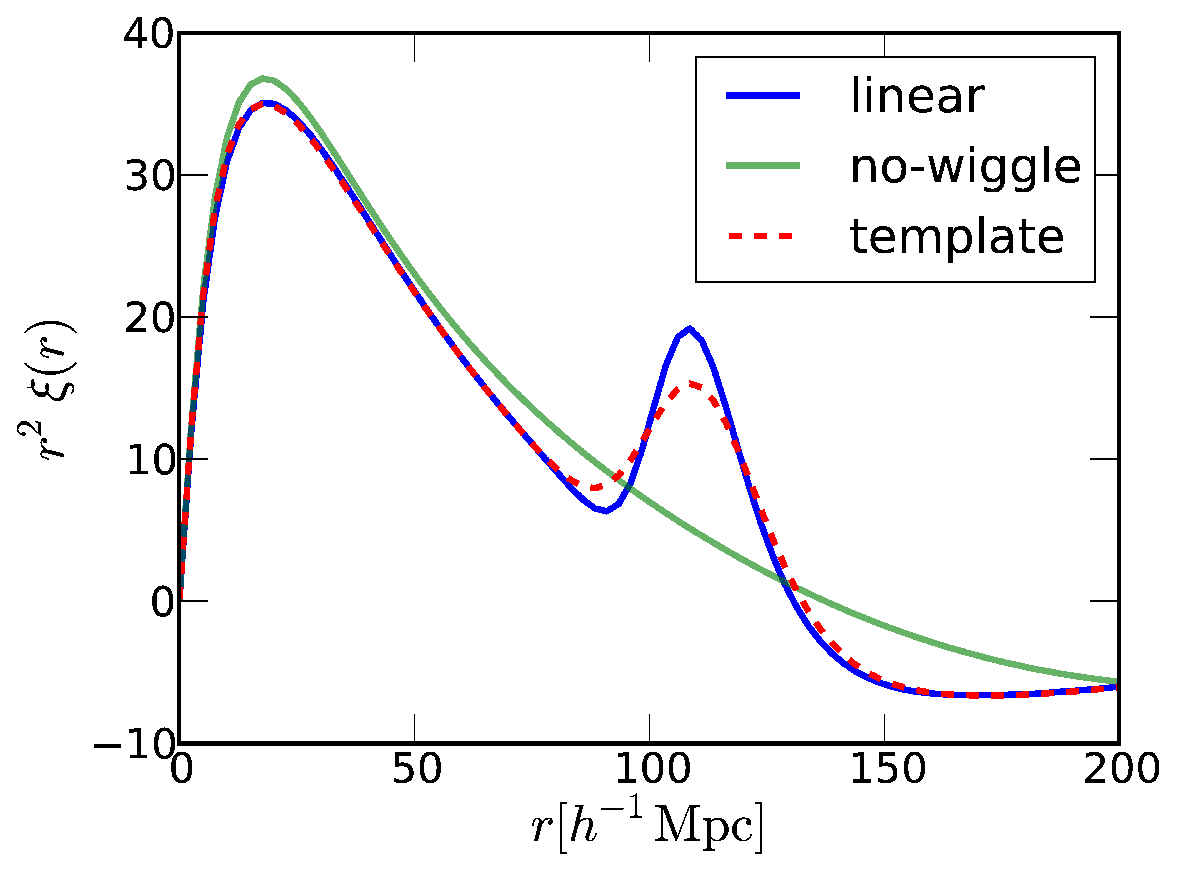
\includegraphics[width=0.5\textwidth]{/Users/old_ts485/Desktop/my_thesis/plots_BAO/xi_template}

\caption{\label{fig:template_fn}Components of the template correlation function
given in Eq. \ref{eq:model1}. The linear correlation function (blue)
and the no-wiggle term (green) are shown as solid lines, while the
template function combining these two terms with $\Sigma=7.5h^{-1}{\rm Mpc}$
is shown as a red dashed line.}


\end{figure}


The parameter $\alpha$ measures the shift in the BAO scale relative
to what is assumed for the template function, and is defined by 
\begin{equation}
\alpha\equiv\left(\frac{D_{{\rm V}}(z)}{r_{{\rm d}}}\right)\left(\frac{r_{{\rm d,fid}}}{D_{{\rm V}}^{{\rm fid}}(z)}\right),\label{eq:alpha_ratio}
\end{equation}
where $r_{{\rm d}}$ is the sound horizon\textcolor{black}{{} at the
drag epoch (i.e., the time at which the baryons are released from
the Compton drag of the photons and the baryon optical depth becomes
one)} and 
\begin{equation}
D_{{\rm V}}\equiv\left[cz(1+z)^{2}D_{{\rm A}}(z)^{2}H^{-1}(z)\right]^{1/3}
\end{equation}
with $D_{{\rm A}}$ being the angular diameter distance and $H(z)$,
the Hubble parameter. In the absence of systematics, we expect $\alpha=1$;
deviations from this represent a systematic bias to the inferred distance-redshift
relation.


\section{Results for Isotropic BAO \label{sec:isotropic}}

In this section, we show the results of the isotropic BAO analysis
with and without reconstruction using the method discussed in Sec.
\ref{sub:fitting}. The HOD parameters used to generate various galaxy
samples and the details of the samples are shown in Table \ref{tab:hod}.
We use the samples generated from the ``weighted'' HOD method in
order to remove the variance on the shift of the BAO peak due to randomly
subsampling halos, which is particularly large for the samples with
high biases. We evaluate the acoustic scale using the parameter $\alpha$,
which measures the shift of the BAO peak. $\alpha=1$ implies that
there is no shift in the BAO scale and therefore the measured cosmology
is the same as the fiducial cosmology.

We discuss the effect of subsampling and compare the results between
the regular HOD and ``weighted'' HOD methods in Sec. \ref{sub:weightHOD}.
In the next two sections, we show the effect of galaxy bias on the
BAO measurements without and with reconstruction. In the last section,
we discuss the effects of various steps on the robustness of the reconstruction.

\begin{table}
\begin{tabular}{|c|c|c|c|c|c|}
\hline 
 & $M_{{\rm cut}}$ & bias & $\bar{n}[h^{3}{\rm Mpc^{-3}}]$ & $R[h^{-1}{\rm Mpc}]$ & $\Sigma[h^{-1}{\rm Mpc}]$\tabularnewline
\hline 
\hline 
HOD1 & 12.5 & 1.314 & $1\times10^{-3}$ & $10h^{-1}{\rm Mpc}$ & $2.5h^{-1}{\rm Mpc}$\tabularnewline
\hline 
HOD2 & 12.7 & 1.364 & $8.17\times10^{-4}$ & $15h^{-1}{\rm Mpc}$ & $3.3h^{-1}{\rm Mpc}$\tabularnewline
\hline 
HOD3 & 12.9 & 1.449 & $6.20\times10^{-4}$ & $15h^{-1}{\rm Mpc}$ & $3.3h^{-1}{\rm Mpc}$\tabularnewline
\hline 
HOD4 & 13.1 & 1.568 & $4.40\times10^{-4}$ & $15h^{-1}{\rm Mpc}$ & $3.3h^{-1}{\rm Mpc}$\tabularnewline
\hline 
HOD5 & 13.3 & 1.715 & $2.95\times10^{-4}$ & $15h^{-1}{\rm Mpc}$ & $3.1h^{-1}{\rm Mpc}$\tabularnewline
\hline 
HOD6 & 13.5 & 1.915 & $1.88\times10^{-4}$ & $20h^{-1}{\rm Mpc}$ & $4.1h^{-1}{\rm Mpc}$\tabularnewline
\hline 
HOD7 & 13.7 & 2.161 & $1.15\times10^{-4}$ & $20h^{-1}{\rm Mpc}$ & $4.8h^{-1}{\rm Mpc}$\tabularnewline
\hline 
HOD8 & 13.9 & 2.434 & $6.74\times10^{-5}$ & $25h^{-1}{\rm Mpc}$ & $4.9h^{-1}{\rm Mpc}$\tabularnewline
\hline 
HOD9 & 14.1 & 2.756 & $3.73\times10^{-5}$ & $30h^{-1}{\rm Mpc}$ & $5.5h^{-1}{\rm Mpc}$\tabularnewline
\hline 
\end{tabular}

\caption{\label{tab:hod}Halo Occupation Distributions and their properties}
\end{table}



\subsection{Comparison between weighted and regular HOD methods\label{sub:weightHOD}}

In this section, we compare the $\alpha$ values measured through
the samples using the regular and ``weighted'' HOD methods to show
how the shot noise affects the measurements.

Fig. \ref{fig:variation_hod} shows the comparison between the $\alpha$
values measured from the regular HOD and ``weighted'' HOD samples.
For the case of the ``weighted'' HOD method, we first compute the
correlation functions with the given weights and measure the $\alpha$
values for the 64 samples denoted as $\alpha_{w}$. For the regular
HOD samples, we generate three different realizations (in total of
192 samples) with ${\rm log_{10}M_{{\rm cut}}=12.5}$ (labeled as
the $HOD1$ samples) and five realizations (in total of 320 samples)
with ${\rm log}_{10}M_{{\rm cut}}=14.1$ (labeled as the $HOD9$ samples),
and measure the shifts denoted as $\alpha$. Then, we compare the
differences in the corresponding $\alpha$ values between the regular
and ``weighted'' HOD samples. For both cases, the mean of the difference
$<\alpha-\alpha_{w}>$ is $\pm0.02\%$. The error of the mean for
the case of the $HOD1$ samples is $0.45\%$, while it is $2.44\%$
for the case of the $HOD9$ samples. With relatively small number
of realizations, the mean alpha values, $<\alpha-1>$, can very from
$0.3\%$ to $1\%$ for the case of $HOD9$, although we expect the
value of $\alpha$ to converge to $\alpha_{w}$ with a larger number
of realizations. 

\begin{figure}[H]
\includegraphics[width=0.45\textwidth]{/Users/old_ts485/Desktop/my_thesis/plots_BAO/comparison_alpha_hod1}\includegraphics[width=0.45\textwidth]{/Users/old_ts485/Desktop/my_thesis/plots_BAO/comparison_alpha_hod9}

\caption{\label{fig:variation_hod}Distribution of the values $\alpha_{HOD}-\alpha_{{\rm weighted}}$
for the case of ${\rm log_{10}}M_{{\rm cut}}=12.5$ (left) and ${\rm log_{10}}M_{{\rm cut}}=14.1$
(right). The green solid lines are the Gaussian fits, where the values
of mean and the standard deviation are shown in the figures. The high
biased samples (in this case the samples with ${\rm log_{10}}M_{{\rm cut}}=14.1$)
have a larger standard deviation, because the larger $M_{{\rm cut}}$
value means more variations in subsampling halos.}
\end{figure}



\subsection{Effects of Biased Tracers on BAO Peaks in Real-Space before Reconstruction
\label{sub:real-prerecon}}

In this section, we investigate the effect of galaxy bias on the measurement
of the BAO peak without reconstruction. We use the method described
in Sec. \ref{sub:fitting} to measure the shift of the BAO peak. The
non-linear parameter in the template function (defined in Eq. \ref{eq:model2})
used for the analysis is $\Sigma=7.5h^{-1}{\rm Mpc}$ for all the
galaxy samples. Since the shifts due to galaxy bias and due to the
deviation from the fiducial cosmology are indistinguishable, it is
important to understand how much systematic biases are induced by
galaxy biases.

Fig. \ref{fig:alpha_prerecon} shows the measured shifts on the BAO
scale as a function of galaxy bias. The $\alpha$ measured for the
HOD samples are given in Table \ref{tab:alphas}. We detect the shift
in the BAO scale ($\sim3\sigma$ for most samples) but do not detect
a strong variation with the galaxy bias. Indeed, the shift is consistent
with being constant for biases $<$ 2.0 and only increases for extremely
large biases. These results agree with the trends shown in Ref. \cite{2011ApJ...734...94M}.
The absolute values of shifts for our samples are larger than the
shifts measured in Ref. \cite{mehta2011}. This is because we use
the samples at a lower redshift. In fact, the size of the increase
in shifts is roughly consistent with the expectations from perturbation
theory \cite{2008PhRvD..77b3533C,2009PhRvD..80f3508P,2012PhRvD..85j3523S}.
The $\alpha-1$ value is proportional to $D^{2}(z)$, where $D(z)$
is the linear growth rate. However, we find that the bias dependence
of our samples is weaker than what was predicted in Ref. \cite{2009PhRvD..80f3508P}.
\textcolor{red}{Note that we use different HOD models than the one
used in Ref. \cite{2009PhRvD..80f3508P}, which give different higher-order
biases in perturbation theory. Since the shift of the BAO peak is
due to higher-order terms (e.g., \cite{2012PhRvD..85j3523S,2009PhRvD..80f3508P}),
the reason we see the weaker dependence on biases is possibly due
to different HOD models.}

\begin{figure}[H]
\includegraphics[width=0.5\textwidth]{/Users/old_ts485/Desktop/my_thesis/plots_BAO/alpha_bias_pre_r_weighted}

\caption{\label{fig:alpha_prerecon}Shift in the BAO scale for the weighted
samples as a function of galaxy bias. Note that $\alpha=1$ (dashed
line) implies no shift in the BAO scale. }


\end{figure}


In order to understand the correlation in the $\alpha$ values between
different galaxy samples, we compare the $\alpha$ values measured
from the samples with ${\rm log}_{10}M_{{\rm cut}}=12.9$ and $14.1$
(corresponding to the galaxy bias of $1.5$ and $2.8$ and denoted
as HOD3 and HOD9 respectively) to the samples with the lowest galaxy
bias (i.e., $\log_{10}M_{{\rm cut}}=12.5$ denoted as HOD1). In Fig.
\ref{fig:scatter_prerecon}, we plot every $\alpha$ value measured
from each sample ($4(h^{-1}{\rm Gpc})^{3}$ each and 64 samples in
total). From the figure, we see that there is a correlation between
the shifts measured for the HOD1 and HOD3 samples and its cross-correlation
coefficient is $0.919$. On the other hand, there is little correlation
for the $\alpha$ values between HOD1 and HOD9 (where the cross-correlation
coefficient is $0.136$) due to a large shot noise.

\begin{figure}[H]
\includegraphics[width=0.45\textwidth]{/Users/old_ts485/Desktop/my_thesis/plots_BAO/alpha_hod1_hod3_pre_r}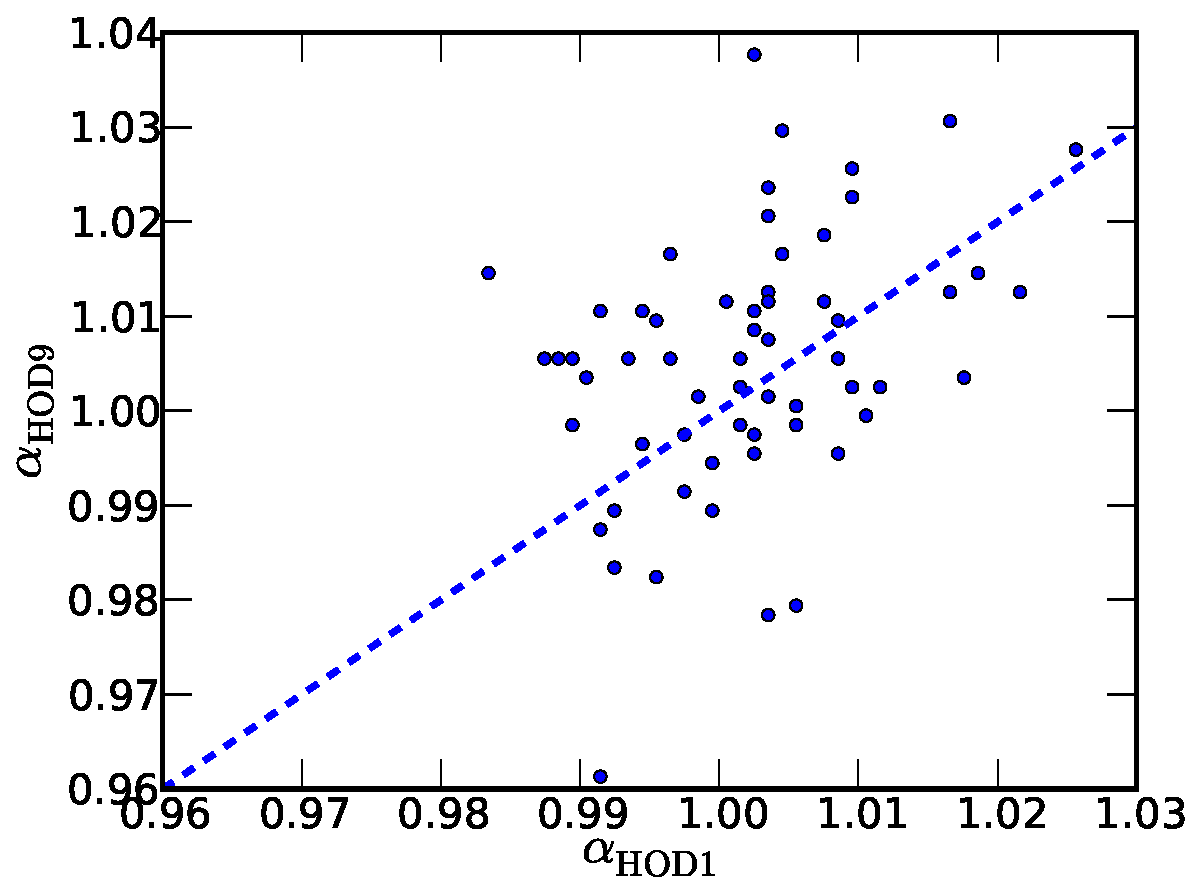
\includegraphics[width=0.45\textwidth]{/Users/old_ts485/Desktop/my_thesis/plots_BAO/alpha_hod1_hod9_pre_r}

\caption{\label{fig:scatter_prerecon}Comparison of the $\alpha$ values for
the samples with ${\rm log}_{10}M_{{\rm cut}}=12.9$ denoted as HOD3
(left) and ${\rm log}_{10}M_{{\rm cut}}=14.1$ denoted as HOD9 (right)
with respect to ${\rm log_{10}}M_{{\rm cut}}=12.5$ denoted as HOD1.
While the cross correlation coefficient between HOD1 and HOD3 is 0.919,
the cross correlation is 0.136 between HOD1 and HOD9.}
\end{figure}


There are three possible sources for the biases and the scatter in
the $\alpha$ measurements. The initial conditions (no biases, but
scatter),\textcolor{red}{{} }\textcolor{black}{the matter density field
(biases due to the non-linear evolution of structure), and the galaxy
populations (biases due to galaxy biases in addition to the non-linear
evolution of structure)}. The first two are common to all the samples
we consider; however, the last one (i.e., galaxy bias) is not. Knowing
that the $\alpha$ values between two samples are correlated for low
biased samples, as shown in Fig. \ref{fig:scatter_prerecon}, we investigate
how biases and scatter are reduced by computing the differences in
the $\alpha$ values, which will tell us the additional biases and
scatter induced by galaxy bias. To test this, we take the $HOD1$
sample as a reference (denoted its $\alpha$ value as $\alpha_{ref}$)
and measure the differences in the $\alpha$ values with the other
samples. Fig. \ref{fig:diffalpha_prerecon} shows the differences
in shift $\alpha_{HOD}-\alpha_{ref}$ for various HOD models corresponding
to different biases. The $\alpha_{HOD}-\alpha_{ref}$ values for each
HOD sample are given in Table \ref{tab:alpha_diff}. As expected from
Fig. \ref{fig:scatter_prerecon}, the scatter is reduced from $0.1\%$
to less than $0.05\%$ for the samples with $b<2$. On the other hand,
for high biases samples, the biases are reduced by $0.3\%$ while
the scatters are almost the same. This is due to the lack of correlation
shown in Fig. \ref{fig:scatter_prerecon}.

\begin{figure}[H]
\includegraphics[width=0.5\textwidth]{/Users/old_ts485/Desktop/my_thesis/plots_BAO/alphaDiff_bias_pre_r_weighted}

\caption{\label{fig:diffalpha_prerecon}The differences in shift $\alpha_{HOD}-\alpha_{ref}$
for various HOD models corresponding to different biases. We use the
$HOD1$ sample as a reference. }


\end{figure}



\subsection{Effects of Biased Tracers in Real-Space after Reconstruction \label{sub:real-postrecon}}

Similar to the previous section, we investigate the effect of galaxy
bias on the acoustic scale for \textcolor{black}{the samples applied
the reconstruction method}. To apply the reconstruction method, we
use different smoothing scales $R$ for different galaxy samples,
as shown in Table \ref{tab:hod}. The smoothing scales are determined
based on the average number density of the sample, $\bar{n}$, such
that the smoothing scale becomes larger than $\bar{n}^{-1/3}$. This
is because using the smoothing scale smaller than $\bar{n}^{-1/3}$
includes the modes which are noise-dominated. For fitting, we use
different non-linear parameters (denoted as $\Sigma$ in Table \ref{tab:hod})
for the template function (see Eq. \ref{eq:model2}). The best-fit
non-linear parameter is measured through the fitting method described
in Sec. \ref{sub:fitting}. To do that, we treat the non-linear parameter,
$\Sigma_{{\rm }}$, as a free parameter. The best-fit values are shown
in Table \ref{tab:hod}.

Fig. \ref{fig:alpha_postrecon} shows the measured shifts of the BAO
peak as a function of galaxy bias. The $\alpha$ measured for these
samples are in Table \ref{tab:alphas}. For the samples with biases
$<2.5$, the reconstruction method corrects the shift of the BAO peak
to almost zero within $1\sigma$-deviation. On the other hand, the
reconstruction over-shifts the peak positions for the case of high-biased
objects (i.e., $HOD8$ and $HOD9$ samples). The figure shows a weak
dependence on galaxy bias that the shifts for the higher-biased objects
become more negative. If the shifts for the high-biased objects are
non-zero but positive, it is possible that the reconstruction method
cannot model the bulk flow well enough to remove the effect of the
non-linear evolution on the acoustic scale. However, we get an opposite
result. It is possible that the cause of over-shifting is due to the
noise and the lack of a large enough number of samples. Another important
change after reconstruction is that the scatter in the $\alpha$ values
are dramatically reduced. In particular, the scatters are reduced
to almost half for the low-biased objects, and it is reduced by $\sim25\%$
even for the high-biased objects. This result for the scatters is
consistent with Ref. \cite{mehta2011}, but the size of the scatter
is smaller.

\begin{figure}[H]
\includegraphics[width=0.5\textwidth]{/Users/old_ts485/Desktop/my_thesis/plots_BAO/alpha_bias_post_r_weight_sigma}

\caption{\label{fig:alpha_postrecon} Shift in the BAO scale after reconstruction
as a function of galaxy bias. Note that $\alpha=1$ implies no shift
in the BAO scale. }
\end{figure}


\textcolor{red}{We further explore the cause of the over-shifting
for the case of the $HOD9$ samples. We find that the median value
of the shift, $\widetilde{(\alpha-1)}$, for the $HOD9$ samples is
$-0.151\%$, which is $1\sigma$ away from zero. Fig. \ref{fig:hist_hod9}
shows the distribution of the shifts for the $HOD9$ samples and also
shows that there are some outliers. This makes the mean $\alpha$
value to be smaller than its median value.}

\begin{figure}
\includegraphics[width=0.5\textwidth]{/Users/old_ts485/Desktop/my_thesis/plots_BAO/hist_hod9_alpha_post_r}

\caption{\label{fig:hist_hod9}Distribution of the shift values $\alpha-1$
for the $HOD9$ samples. }


\end{figure}


\textcolor{red}{{*}mention about medians/outliers in HOD9}

To quantify the improvements on the shift of the BAO peak for each
sample, we compare the $\alpha$ values before and after reconstruction
for the $HOD1$ and $HOD9$ samples, as shown in Fig. \ref{fig:scatter_postrecon}.
For the case of the $HOD1$ samples, the improvement after reconstruction
is clear that the scatter in the $\alpha$ values is significantly
reduced. \textcolor{red}{The improvement in the reduction of the scatter
is almost a factor of 2. }On the other hand, the scatter in the $\alpha$
values for the $HOD9$ samples is reduced by $25\%$. 

\begin{figure}[H]
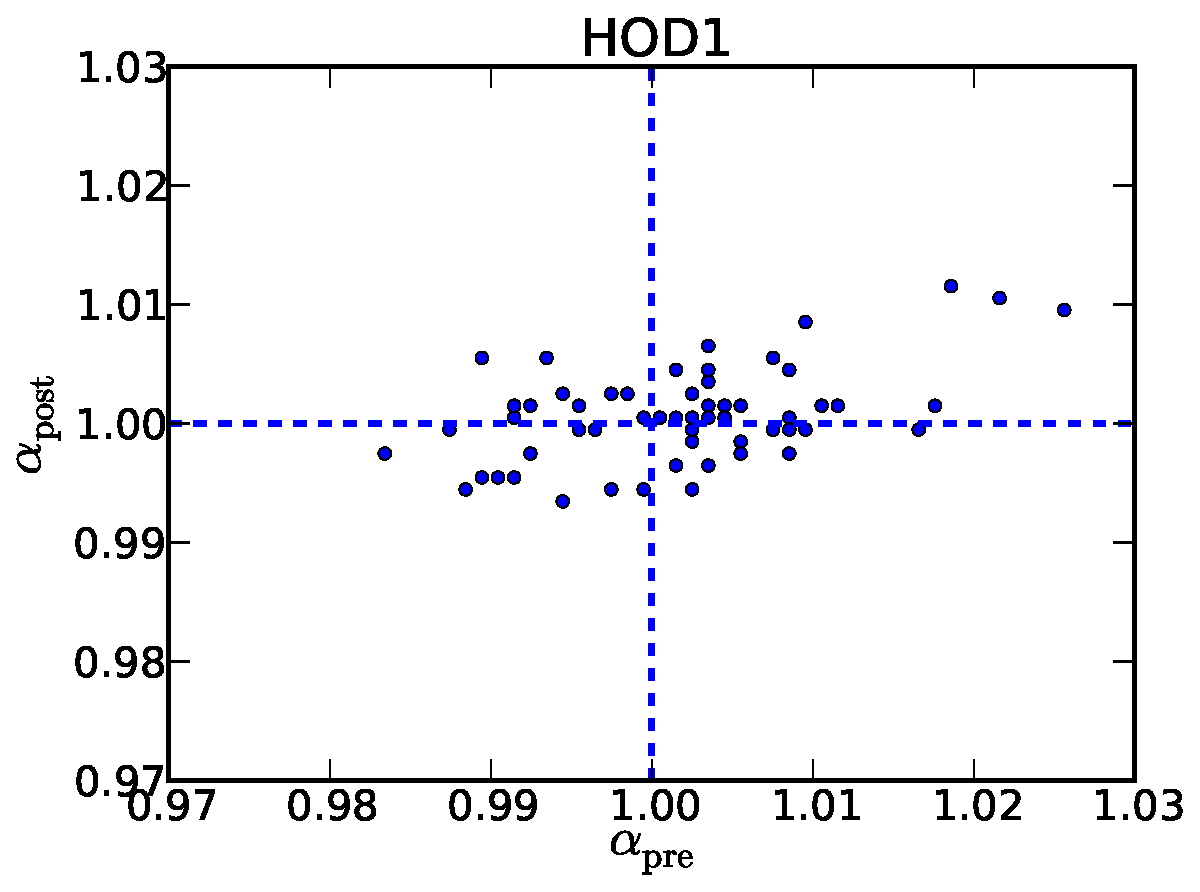
\includegraphics[width=0.45\textwidth]{/Users/old_ts485/Desktop/my_thesis/plots_BAO/alpha_beforeAfter_hod1}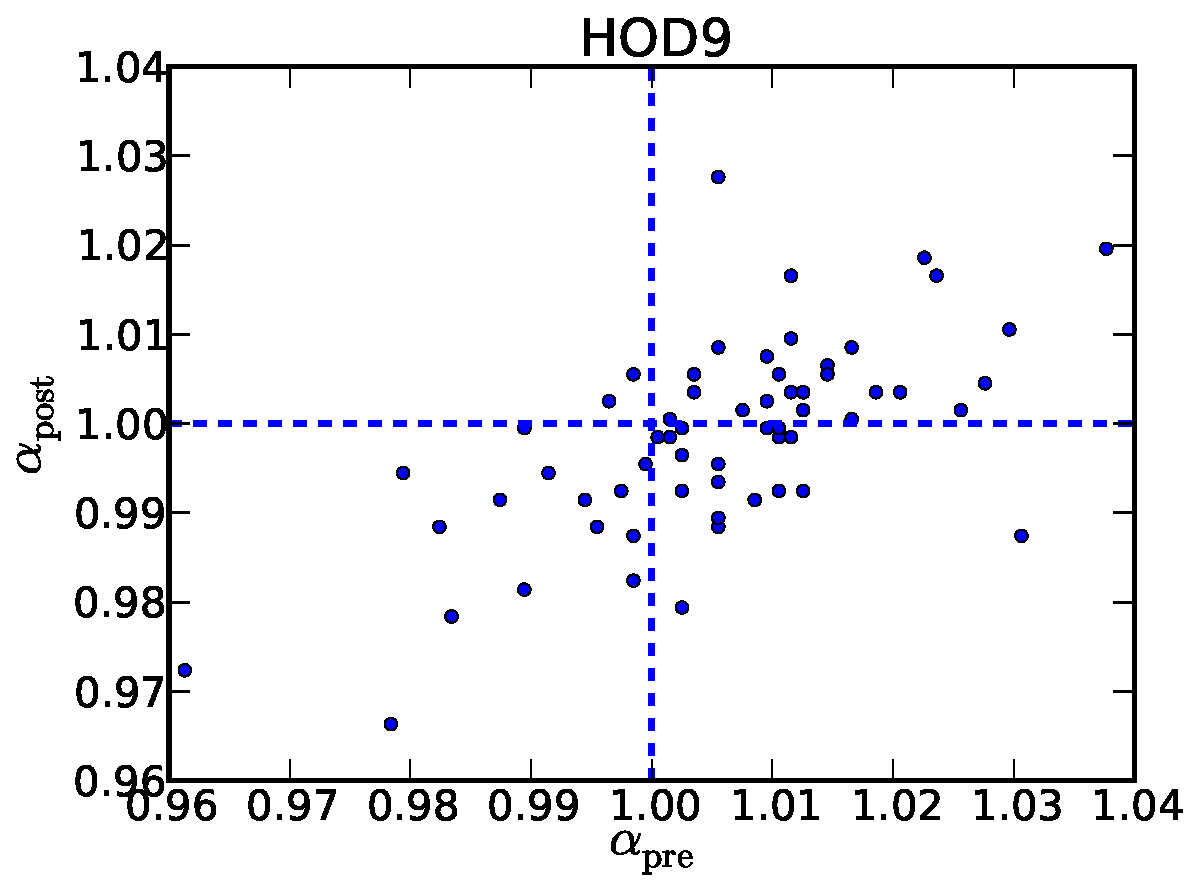
\includegraphics[width=0.45\textwidth]{/Users/old_ts485/Desktop/my_thesis/plots_BAO/alpha_beforeAfter_hod9}

\caption{\label{fig:scatter_postrecon}Comparison of the $\alpha$ values before
and after reconstruction for the $HOD1$ samples (left) and the $HOD9$
samples (right). \textcolor{red}{While the scatter in the $\alpha$
values for the $HOD1$ samples is significantly reduces after reconstruction,
the change of the scatter is little for the case of the $HOD9$ samples.}}
\end{figure}


\begin{table}
\begin{tabular}{|c|c|c|c|c|c|}
\hline 
 & $<\alpha_{{\rm pre}}-1>[\%]$ & $\sigma_{\alpha}[\%]$ & $<\alpha_{{\rm post}}-1>[\%]$ & $\widetilde{(\alpha_{{\rm post}}-1)}[\%]$ & $\sigma_{\alpha}[\%]$\tabularnewline
\hline 
\hline 
$HOD1$ & 0.229 & 0.107 & 0.066 & 0.050 & 0.049\tabularnewline
\hline 
$HOD2$ & 0.261 & 0.103 & 0.031 & -0.050 & 0.063\tabularnewline
\hline 
$HOD3$ & 0.262 & 0.101 & 0.072 & -0.050 & 0.063\tabularnewline
\hline 
$HOD4$ & 0.253 & 0.102 & 0.063 & -0.050 & 0.062\tabularnewline
\hline 
$HOD5$ & 0.273 & 0.103 & 0.0031 & -0.151 & 0.071\tabularnewline
\hline 
$HOD6$ & 0.336 & 0.112 & -0.031 & -0.151 & 0.076\tabularnewline
\hline 
$HOD7$ & 0.396 & 0.120 & -0.095 & -0.151 & 0.090\tabularnewline
\hline 
$HOD8$ & 0.433 & 0.140 & -0.162 & -0.151 & 0.099\tabularnewline
\hline 
$HOD9$ & 0.537 & 0.166 & -0.341 & -0.151 & 0.125\tabularnewline
\hline 
\end{tabular}

\caption{\label{tab:alphas} The $\alpha-1$ values for the HOD samples before
and after the reconstruction method.}


\end{table}


\begin{table}
\begin{tabular}{|c|c|c|c|c|}
\hline 
 & $<\alpha_{{\rm HOD}}-\alpha_{ref}>_{{\rm pre}}[\%]$  & $\sigma_{\alpha,{\rm pre}}[\%]$  & $<\alpha_{{\rm HOD}}-\alpha_{ref}>_{{\rm post}}[\%]$  & $\sigma_{\alpha,{\rm post}}[\%]$ \tabularnewline
\hline 
\hline 
$HOD2$ & 0.031 & 0.023 & -0.035 & 0.030\tabularnewline
\hline 
$HOD3$ & 0.033 & 0.030 & 0.006 & 0.033\tabularnewline
\hline 
$HOD4$ & 0.024 & 0.039 & -0.003 & 0.038\tabularnewline
\hline 
$HOD5$ & 0.044 & 0.053 & -0.063 & 0.051\tabularnewline
\hline 
$HOD6$ & 0.107 & 0.067 & -0.069 & 0.059\tabularnewline
\hline 
$HOD7$ & 0.166 & 0.086 & -0.162 & 0.075\tabularnewline
\hline 
$HOD8$ & 0.204 & 0.118 & -0.228 & 0.091\tabularnewline
\hline 
$HOD9$ & 0.308 & 0.161 & -0.407 & 0.118\tabularnewline
\hline 
\end{tabular}

\caption{\label{tab:alpha_diff} The $\alpha_{{\rm HOD}}-\alpha_{ref}$ values
for the HOD samples using the $HOD1$ sample as a reference.}


\end{table}


In Sec. \ref{sub:real-prerecon}, we investigated the correlation
in the $\alpha$ values between different galaxy samples. We explore
the same thing to see how the correlation in the $\alpha$ values
is changed after reconstruction. To do that, we compare the $\alpha$
values measured from the $HOD3$ and $HOD9$ samples to the $HOD1$
sample. In Fig. \ref{fig:scatter_prerecon}, we plot every $\alpha$
value measured from each sample ($4(h^{-1}{\rm Gpc})^{3}$ each and
64 samples in total). From the figure, we see the same trend as before,
but a weaker correlation. The cross-correlation coefficient between
the $HOD1$ and $HOD3$ samples is 0.719, which is decreased by $\sim20\%$
compared to the correlation for the pre-reconstruction samples. For
the case of the $HOD1$ and $HOD9$ samples, the coefficient is 0.091.
As is clear from the figure, the scatter in the $\alpha$ values for
the $HOD1$ samples is significantly reduced after reconstruction,
while the scatter is almost the same for the case of the $HOD9$ sample.

As a demonstration, Figs. \ref{fig:xi0_hod1} and \ref{fig:xi0_hod9}
plot the correlation functions and the corresponding $\chi^{2}$ distributions
before and after reconstruction using the $HOD1$ and $HOD9$ samples.
The volume of the sample used here is $64(h^{-1}{\rm Gpc})^{3}$.
For both cases, the peaks are clearly sharpened after reconstruction.
However, the chi-square minimum is increased, especially for the case
of the $HOD1$ sample. This is because the template function used
to measure the BAO peak is not as sharp as the reconstructed peak,
which can be fixed by using a different template function. The reason
the minimum chi-square value for the $HOD9$ sample is better than
the one for the $HOD1$ sample is because a less sharpened peak fits
better by the template function. Another important change after reconstruction
is that the chi-square distribution after reconstruction is sharpened,
which implies that the scatter in the $\alpha$ values is reduced. 

\begin{figure}[H]
\includegraphics[width=0.45\textwidth]{/Users/old_ts485/Desktop/my_thesis/plots_BAO/alpha_hod1_hod3_post_r}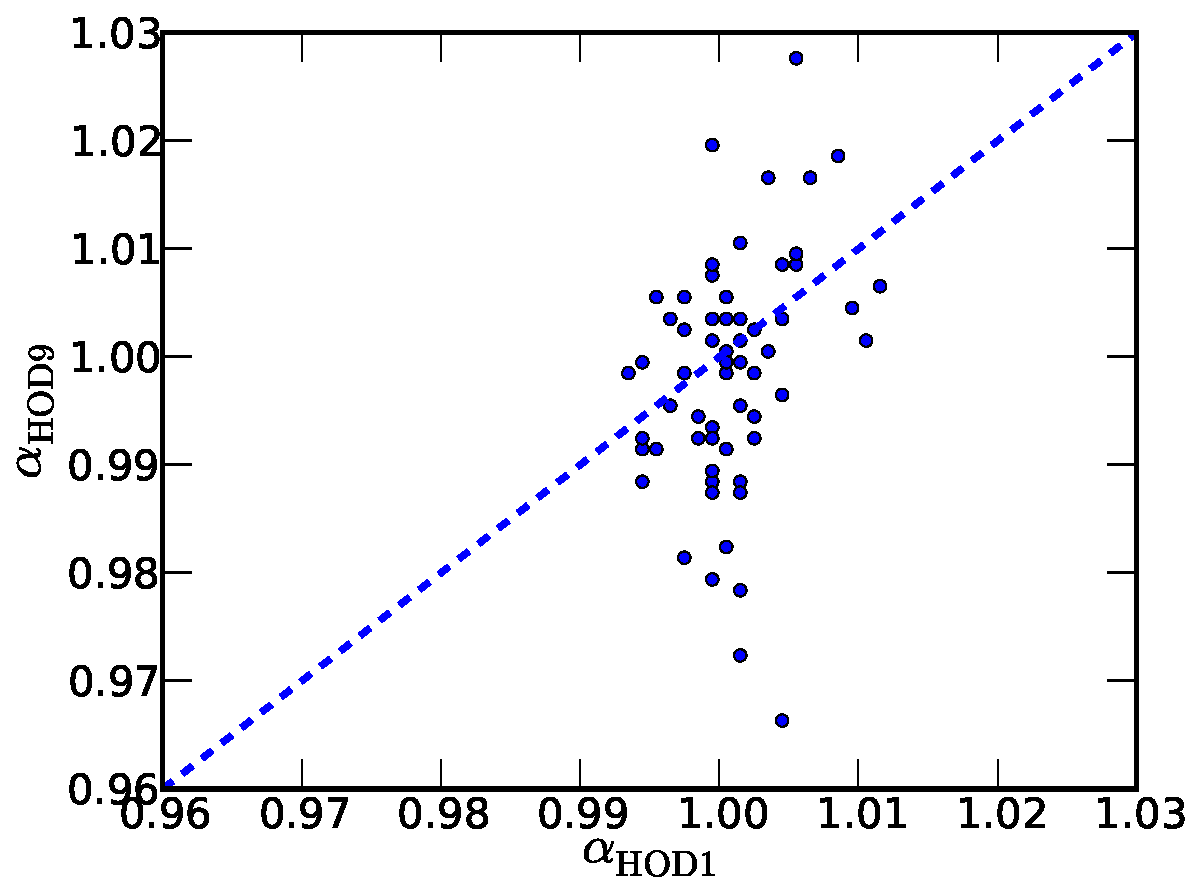
\includegraphics[width=0.45\textwidth]{/Users/old_ts485/Desktop/my_thesis/plots_BAO/alpha_hod1_hod9_post_r}

\caption{\label{fig:scatter_postrecon-1}Comparison of the $\alpha$ values
for the $HOD3$ sample (left) and the $HOD9$ sample (right) with
respect to the $HOD1$ sample. The cross correlation coefficient between
$HOD1$ and $HOD3$ is 0.719, while the cross correlation is 0.091
between $HOD1$ and $HOD9$. }
\end{figure}


\begin{figure}[H]
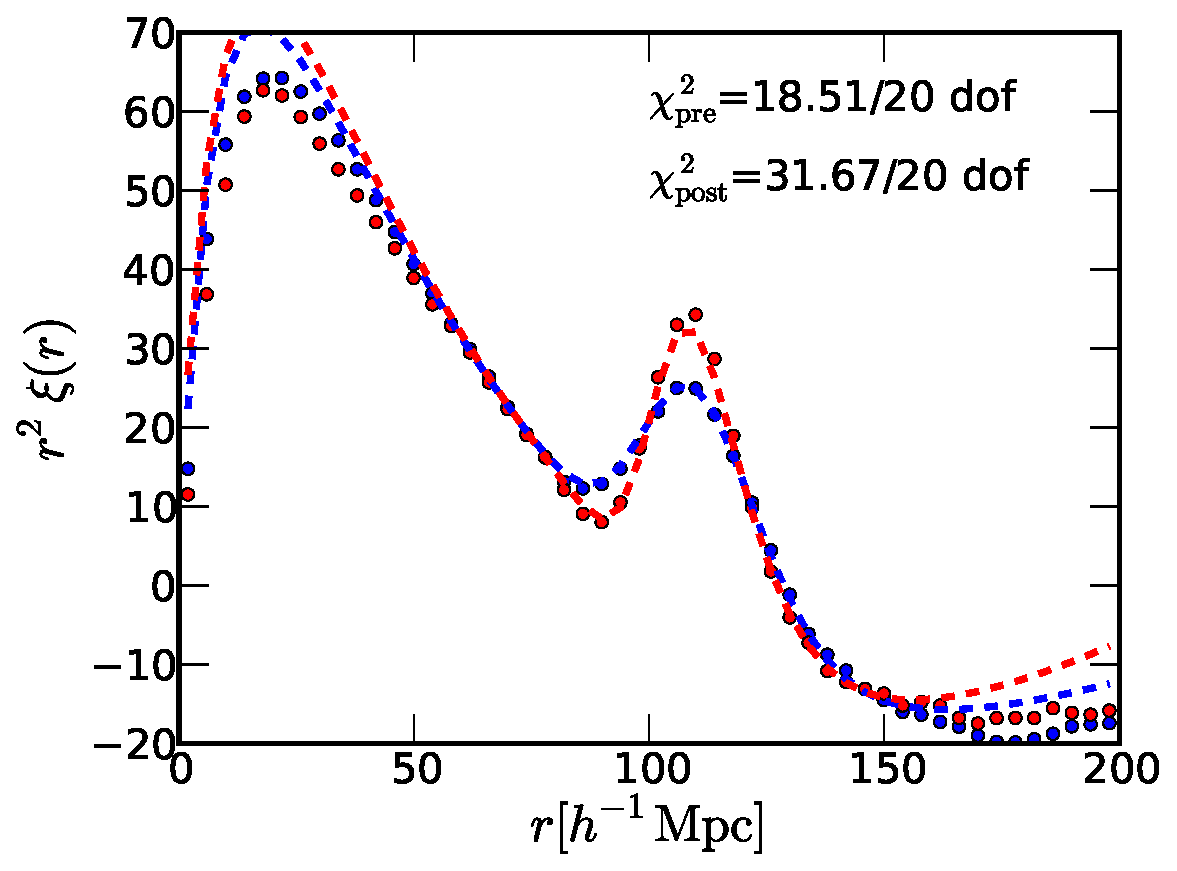
\includegraphics[width=0.5\textwidth]{/Users/old_ts485/Desktop/my_thesis/plots_BAO/hod1_full}\includegraphics[width=0.5\textwidth]{/Users/old_ts485/Desktop/my_thesis/plots_BAO/hod1_full_chi}

\caption{\label{fig:xi0_hod1}Left: The unreconstructed (blue) and reconstructed
(red) correlation functions computed from the $HOD1$ sample. The
error bars are the standard deviation of the four HACC simulations.
Note that we use the samples with the volume of $64(h^{-1}{\rm Gpc})^{3}$.
The solid lines are the best fit model to these data. Right: The $\Delta\chi^{2}$
curve as a function of $\alpha-1[\%]$ before (blue dashed) and after
(red solid) reconstruction.}
\end{figure}


\begin{figure}[H]
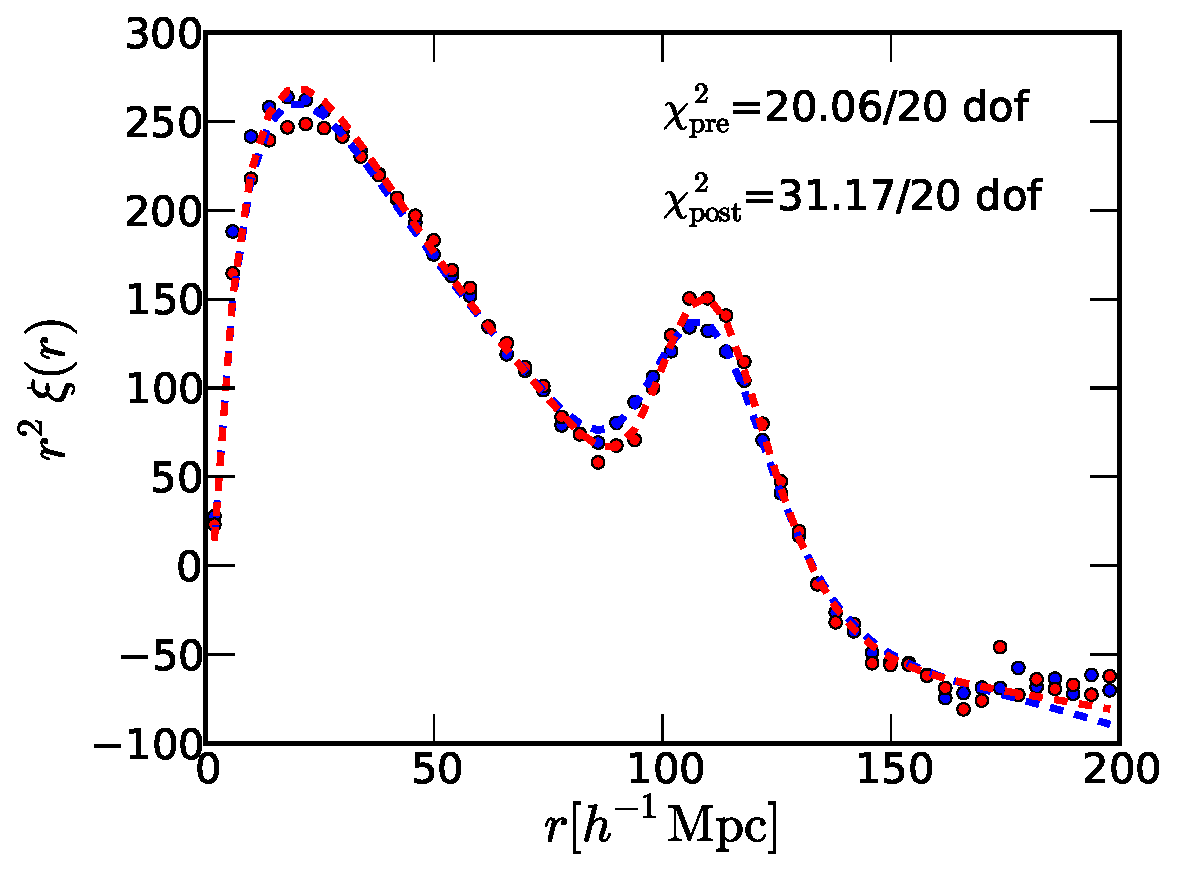
\includegraphics[width=0.5\textwidth]{/Users/old_ts485/Desktop/my_thesis/plots_BAO/hod9_full}\includegraphics[width=0.5\textwidth]{/Users/old_ts485/Desktop/my_thesis/plots_BAO/hod9_full_chi}

\caption{\label{fig:xi0_hod9}Left: The unreconstructed (blue) and reconstructed
(red) correlation functions computed from the $HOD9$ sample. The
error bars are the standard deviation of the four HACC simulations.
Note that we use the samples with the volume of $64(h^{-1}{\rm Gpc})^{3}$.
The solid lines are the best fit model to these data. Right: The $\Delta\chi^{2}$
curve as a function of $\alpha-1[\%]$ before (blue dashed) and after
(red solid) reconstruction.}
\end{figure}



\subsection{Smoothing Scales and Reconstruction}

In this section, we explore the effects of various steps in the reconstruction
method: smoothing scales and noise due to high-biased objects (and
galaxy bias?). We first vary the smoothing scales used to estimate
the linear density field. When the smoothing scale is smaller than
$\bar{n}^{-1/3}$, the reconstructed field is affected by noise due
to the finite number of galaxies. On the other hand, using too large
smoothing scale will degrade the robustness of the method. To test
these effects, we use two galaxy samples $HOD1$ and $HOD9$, which
have two extreme number densities. The number densities for these
samples are $10^{-3}(h^{-1}{\rm Mpc})^{3}$ and $3.73\times10^{-5}(h^{-1}{\rm Mpc})^{3}$,
which correspond to the minimum smoothing scales of $10h^{-1}{\rm Mpc}$
and $30h^{-1}{\rm Mpc}$ respectively. 

For the case of the $HOD1$ sample, we test the effect of large smoothing
scales on the robustness of the method using the smoothing scales
of $10h^{-1}{\rm Mpc}$, $20h^{-1}{\rm Mpc}$, and $30h^{-1}{\rm Mpc}$.
Fig. \ref{fig:hod1_smooth} shows the reconstructed correlation functions
for these smoothing scales. For the case of the large smoothing scales,
the BAO peaks are slightly degraded compared to the correlation function
with the $10h^{-1}{\rm Mpc}$ smoothing scale, but their peaks are
still more sharpened than the case of pre-reconstruction. The measured
shifts on the BAO peak with various smoothing scales are shown in
Table \ref{tab:hod1_smooth}. As the smoothing scale becomes larger,
the scatter on the $\alpha$ values becomes large\textcolor{black}{r.
This is because the correlation in the measured shifts for these samples
becomes smaller. Quantitatively, the cross-correlation coefficients
for the samples with $R=20h^{-1}{\rm Mpc}$ and $30h^{-1}{\rm Mpc}$
with respect to the ones with $R=10h^{-1}{\rm Mpc}$ are $0.71$ and
$0.53$ respectively. In addition to degrading the robustness of the
reconstruction, we find that the reconstructed correlation function
is slightly distorted on small scales by the increase of the smoothing
scales.}

\begin{table}
\begin{tabular}{|c|c|c|}
\hline 
$R$ & $<\alpha-1>[\%]$ & $\sigma_{\alpha}[\%]$\tabularnewline
\hline 
\hline 
$10h^{-1}{\rm Mpc}$ & 0.065 & 0.049\tabularnewline
\hline 
$20h^{-1}{\rm Mpc}$ & -0.019 & 0.075\tabularnewline
\hline 
$30h^{-1}{\rm Mpc}$ & -0.163 & 0.080\tabularnewline
\hline 
\end{tabular}

\caption{\label{tab:hod1_smooth}The effect of the smoothing scales of the
reconstruction on the BAO measurements for the $HOD1$ sample. }
\end{table}


\begin{figure}[H]
\includegraphics[width=0.5\textwidth]{/Users/old_ts485/Desktop/my_thesis/plots_BAO/hod1_xi0_recon_sigmas}

\caption{\label{fig:hod1_smooth}The reconstructed correlation functions using
the $HOD1$ sample with various smoothing scales. Note that the green
line (which shows the correlation function with the $20h^{-1}{\rm Mpc}$
smoothing scale) is almost identical to the one with the $30h^{-1}{\rm Mpc}$
smoothing scale (red).}
\end{figure}


For the case of the $HOD9$ sample, we test the effect of noise on
the reconstructed correlation function. Since the minimum smoothing
scale for the $HOD9$ sample is $30h^{-1}{\rm Mpc}$, using the $10h^{-1}{\rm Mpc}$
smoothing scale includes noise in estimating the ``shifted'' field,
$\vec{s}$. Fig. \ref{fig:hod9_smooth} shows the reconstructed correlation
functions for $HOD9$ sample with the smoothing scales of $10h^{-1}{\rm Mpc}$
and $30h^{-1}{\rm Mpc}$. For the case of the $10h^{-1}{\rm Mpc}$
smoothing scale, even though the peak is sharpened relative to the
case without reconstruction, the shape of the reconstructed correlation
function is distorted on $r\sim50h^{-1}{\rm Mpc}-130h^{-1}{\rm Mpc}$.
However, despite the fact that the reconstructed correlation function
is distorted for the case of the $10h^{-1}{\rm Mpc}$ smoothing scale,
we see little differences in the measure $\alpha$ values compared
to the case of $30h^{-1}{\rm Mpc}$ smoothing scale. The measured
$\alpha-1$ value is $-0.336\pm0.124$ for the case of the $10h^{-1}{\rm Mpc}$
smoothing scale and $-0.311\pm0.126$ for the case of the $30h^{-1}{\rm Mpc}$
smoothing scale. This indicates that the distortion of the correlation
functions on small scales has little impact on the measurement of
the BAO peak.

\begin{figure}[H]
\includegraphics[width=0.5\textwidth]{/Users/old_ts485/Desktop/my_thesis/plots_BAO/hod9_xi0_recon_sigmas}

\caption{\label{fig:hod9_smooth}Analogous to Fig. \ref{fig:hod1_smooth},
but using the $HOD9$ sample with the smoothing scales of $10h^{-1}{\rm Mpc}$
and $30h^{-1}{\rm Mpc}$. The minimum smoothing scale for the $HOD9$
sample is $30h^{-1}{\rm Mpc}$, which means that using the $10h^{-1}{\rm Mpc}$
smoothing scale includes the noise in the estimation of the ``shifted''
field defined in Eq. \ref{eq:shifted_field}. The dashed line is the
correlation function without reconstruction.}
\end{figure}


In order to quantify the effect of galaxy bias on the estimation of
the shifted field, we use the $HOD1$ samples to estimate the shifted
field, $\vec{s}$, to do the reconstruction for the $HOD9$ samples.
Since the $HOD1$ samples have smaller galaxy biases, the distribution
of the galaxies in the $HOD1$ samples is a better representation
of the underlying DM density field. For reconstruction, we use the
smoothing scale of $\Sigma=10h^{-1}{\rm Mpc}$. Fig. \ref{fig:recon_hod1to9}
shows the reconstructed correlation functions using the $HOD1$ and
$HOD9$ samples to estimate $\vec{s}$. The BAO peak is more sharpened
when $\vec{s}$ is computed from the $HOD1$ samples. Note that this
sharpening is not due to using different smoothing scales. As shown
in Fig. \ref{fig:hod9_smooth}, using smaller smoothing scale for
the $HOD9$ samples does not improve the sharpening. In addition to
the improvement in the shape of the BAO peak, the measured $\alpha-1$
values are improved from $(-0.341\pm0.125)\%$ to $(-0.116\pm0.116)\%$
by using the $HOD1$ samples. This implies that the systematic bias
is reduced from $\sim3\sigma$ deviation to about a $1\sigma$ deviation. 

\begin{figure}[H]
\includegraphics[width=0.5\textwidth]{/Users/old_ts485/Downloads/hod9_xi0_recon_switch}

\caption{\label{fig:recon_hod1to9}Reconstructed correlation functions for
the $HOD9$ samples. The blue line shows the correlation function
using the $HOD9$ samples to estimate the ``shifted'' field, while
the green line shows the correlation function using the $HOD1$ samples.}
\end{figure}


In addition to compute the reconstructed correlation functions using
different ``shifted'' fields, we compare these fields by projecting
onto the galaxies in the $HOD9$ samples. We first compute the ``shifted''
fields from the $HOD1$ and $HOD9$ samples. Then, we shift the positions
of the galaxies in the $HOD9$ samples using these estimated fields
respectively. We take the differences in the positions of the corresponding
galaxies. Fig. \ref{fig:pos_hod1to9} shows the differences in the
shifted positions using the $HOD1$ and $HOD9$ samples. There are
two causes for having different ``shifted'' fields. One is due to
different galaxy biases, and the other is due to different smoothing
scales. To know how much difference is introduced by these causes,
we compute the ``shifted'' field from the $HOD1$ samples using
two different smoothing scales, $10h^{-1}{\rm Mpc}$ and $30h^{-1}{\rm Mpc}$.
Note that we use the $30h^{-1}{\rm Mpc}$ smoothing scale to compute
$\vec{s}$ from the $HOD9$ samples. The standard deviations in the
differences are $\sim1.5h^{-1}{\rm Mpc}$ for the case of the $30h^{-1}{\rm Mpc}$
smoothing scale and $\sim2.7h^{-1}{\rm Mpc}$ for the case of the
$10h^{-1}{\rm Mpc}$ smoothing scale. For the case of the $30h^{-1}{\rm Mpc}$
smoothing scale, the differences are mainly due to the large noise
of the $HOD9$ samples. On the other hand, some of the difference
comes from including more modes to estimate $\vec{s}$ for the case
of the $10h^{-1}{\rm Mpc}$ smoothing scale.

\begin{figure}[H]
\includegraphics[width=0.5\textwidth]{/Users/old_ts485/Desktop/my_thesis/plots_BAO/hist_x_on_hod9}

\caption{\label{fig:pos_hod1to9}Comparison of the shifted positions of the
galaxies in the $HOD9$ samples. We estimate the ``shifted'' field
using the $HOD1$ and $HOD9$ samples and shift the positions of galaxies
accordingly. Then, we compare the differences in the positions of
the corresponding galaxies. Different colors correspond to the smoothing
scale used to the $HOD1$ samples to estimate $\vec{s}$.}
\end{figure}


As a final test, we compute cross-correlation functions between the
$HOD1$ and $HOD9$ samples to see the change in the measured $\alpha$
values. Fig. \ref{fig:cross} shows the measured shifts of the BAO
peak as a function of galaxy bias before and after reconstruction.
The $\alpha$ measured from the cross correlation functions are plotted
in red. Both measured bias and $\alpha$ values are \textcolor{red}{almost
the mean values between the $HOD1$ and $HOD9$ samples. Ref. \cite{2009PhRvD..80f3508P}
shows that $P_{22}$ (the auto power spectrum of the second-order
term $\delta^{(2)}$ in perturbation theory) gives the out-of-phase
contribution in the non-linear power spectrum, which causes the shift
of the BAO peak. The shifted power spectrum $P_{L}(k/\alpha)$ is
Taylor expanded such as 
\[
P_{L}(k/\alpha)\simeq P_{L}(k)-(\alpha-1)\frac{dP_{L}}{d{\rm ln}k}+\cdots,
\]
where $P_{L}$ is the linear power spectrum. The $P_{22}$ term well
approximates the log-derivative of the power spectrum $dP_{L}/d{\rm ln}k$.
Using the above equation, if the $HOD1$ and $HOD9$ samples are not
correlated, the $P_{22}$ term for the $ $cross power spectrum is
proportional to $(1-\frac{1}{2}\alpha_{HOD1}-\frac{1}{2}\alpha_{HOD9}+\cdots)\frac{dP_{L}}{d{\rm ln}k}$.
Therefore, the measured $\alpha$ values for the cross-correlation
functions are consistent with what is expected in perturbation theory.
Furthermore, the cross-correlation functions after reconstruction
corrects the shift of the BAO peak properly even when cross-correlating
with the $HOD9$ samples which are over-shifted due to noise. This
implies that we can use the low number density samples to measure
the BAO peak by cross-correlating with the high number density samples.}

\begin{figure}[H]
\includegraphics[width=0.5\textwidth]{/Users/old_ts485/Desktop/my_thesis/plots_BAO/alpha_bias_pre_r_weighted2}\includegraphics[width=0.5\textwidth]{/Users/old_ts485/Desktop/my_thesis/plots_BAO/alpha_bias_post_r_weighted2}

\caption{\label{fig:cross}Left: Shift in the BAO scale for the cross correlation
functions between the $HOD1$ and $HOD9$ samples (red points) before
reconstruction as a function of galaxy bias. Right: Similar to the
left figure but after reconstructions. The blue points are from the
HOD samples listed in Table \ref{tab:hod}.}
\end{figure}



\section{Discussion \label{sec:Discussion}}

In this study, we present the effects of galaxy bias on the BAO measurements
using high-resolution N-body simulations with the volume of $256(h^{-1}{\rm Gpc})^{3}$
at $z=0.15$, which is a lower redshift than the redshift tested in
Ref. \cite{mehta2011}. We use the HOD method to simulate various
galaxy populations. We also explore the robustness of the reconstruction
methods by varying the smoothing scales as well as by estimating the
``shifted'' fields using different samples.

We conclude this chapter with the following summary of our findings.
\begin{enumerate}
\item We find that the effect of shot noise is particularly large on high-biased
objects, and therefore decide to use the samples generated from the
``weighted'' HOD method, which removes the variance on the shift
of the BAO peak due to randomly subsampling halos.
\item For the case of pre-reconstruction, we detect the shift in the BAO
scale ($\sim3\sigma$ for most samples), which is consistent with
the expectations from perturbation theory \cite{2008PhRvD..77b3533C,2009PhRvD..80f3508P,2012PhRvD..85j3523S}.
The shift is consistent with being constant for biases $<$ 2.0 and
only increases for extremely large biases, as is seen in Ref. \cite{mehta2011}.
However, we do not find the strong bias dependence predicted in Ref.
\cite{2009PhRvD..80f3508P}. 
\item For the case of post-reconstruction, the reconstruction method corrects
the shift of the BAO peak to almost zero within $1\sigma$-deviation
for most samples and reduces the scatter in the measured $\alpha$
values by a factor of $1.5-2$. However, the reconstruction over-shifts
the peak positions for the case of high-biased objects ($b>2.5$),
and the reduction of the scatter is not as effective as for the low-biased
samples.
\item Using the $HOD1$ samples to estimate the ``shifted'' field for
the reconstruction to the $HOD9$ samples, the shift and the scatter
of the BAO peak are significantly improved. We find that the reconstruction
corrects the shift to almost zero within $1\sigma$, which is an improvement
from $3\sigma$ deviations. This implies that having large noise in
the samples can induce over-shifting when the reconstruction method
is applied.
\item We find that using a larger smoothing scale increases the scatters
in the measured $\alpha$ values, but does not affect the peak position
unless it is too extreme.
\end{enumerate}
As a possible direction for future work, we can investigate the effects
of galaxy bias on the BAO scale in redshift-space. For the case of
redshift-space, we can utilize the anisotropy due to the Alcock-Paczynski
effect to fully constrain $D_{A}(z)$ as well as $H(z)$. In addition
to extending this work to redshift-space, we can explore how the reconstruction
method affects higher-order terms in perturbation theory. In particular,
we can utilize the second-order term, which is responsible for the
shift and the broadening of the BAO peak, to quantify the robustness
of the reconstruction method.

{*}using different cosmology and redshift

{*}using different satellite fraction; give weights similar to abundance
matching

{*}using the samples at different redshift to do reconstruction

{*}using higher-order term to quantitatively evaluate the reconstruction
method


\section{Appendix}


\subsection{Things to study}

{*}Fisher matrix analysis for future...

{*}mention about that the difference in s-field is nothing

{*}correlation between smoothing scale and number density -> mention
how smoothing scale affects to the shift in alpha and also the shape
of dd...

{*}shot noise

{*}correlation length

{[}Is drag epoch and decoupling the same?: The decoupling epoch is
when the photon optical depth is one. The drag epoch is when the baryon
optical depth is one. Since there are many more photons than baryons,
the photons \textquotedbl{}decouple\textquotedbl{} (stop noticing
the baryons) before the baryons stop noticing the photons.{]}

{[}the reason the redshift-evolution of $r_{d}$ is proportional to
$1/D_{V}$ {]}

{[}ask about eq. 7 in Noh et al... how $\Sigma^{2}$ is related to
the smoothing scales...{]}

{[}ask about how to estimate the scatter from the size of the shot
noise{]}

{[}lookbacktime/ redshift and the corresponding physical time{]}

{[}unit of pc/solar masses{]}


\subsection{Effects of Smoothing Scales\label{sub:smoothing}}

In this section, we discuss how the smoothing parameter $\Sigma$
in the template correlation function affects the measurement of $\alpha$.
The expected value for $\Sigma$ is xxx, which is computed from xxx.
We use the sample with $\log_{10}M_{{\rm cut}}=12.5$. For each set
of samples ($4(h^{-1}{\rm Gpc})^{3}$ each and 64 samples in total),
we change the value of $\Sigma$ and measure the $\alpha$ value.

Fig. \ref{fig:sigma_prerecon} shows the values of $\alpha$ and the
corresponding $\chi^{2}$ values as a function of various values for
the smoothing parameter in real-space before reconstruction. While
decreasing the smoothing scale makes the shift of the BAO peak smaller
monotonically, the $\chi^{2}$ values indicate that $\Sigma=7.5h^{-1}{\rm Mpc}$
gives the smallest value and therefore the best fit. We repeat the
same exercises for different HOD samples (i.e., different galaxy biases)
and for the case of post-reconstruction. For the case of samples with
various HOD parameters, we did not see any bias-dependence on the
smoothing scales. For the case of post-reconstruction, the smoothing
scale which gives the smallest $\chi^{2}$ value is $\Sigma=2.5h{\rm Mpc}$,
which is much smaller than what we expected. {[}\textcolor{red}{explain
what we expected and why it's a reasonable thing to expect}{]} \textcolor{black}{While
the smoothing scale $\Sigma$ really changes the $\alpha$ value for
the case of pre-reconstruction, the $\alpha$ value does not show
significant changes for the case of post-reconstruction. }{[}\textcolor{red}{possible
reasons? and also is this a correct statement to make?}if so, put
more quantitative values.{]}

{*}Also, mention somewhere about the results when I vary $\Sigma$
and the best fit value of $\Sigma$

\begin{figure}[H]
\includegraphics[width=0.45\textwidth]{/Users/old_ts485/Desktop/my_thesis/plots_BAO/alpha_sigma_hod1_pre_r}\includegraphics[width=0.45\textwidth]{/Users/old_ts485/Desktop/my_thesis/plots_BAO/chiSquare_sigma_hod1_pre_r}

\caption{\label{fig:sigma_prerecon}(regenerate the plot) $<\alpha-1>$ (left)
and $<\chi^{2}>$ (right) as a function of smoothing scale $\Sigma$.
In order to measure the $\alpha$ value, we use the sample with $\log_{10}M_{{\rm cut}}=12.5$
before reconstruction. We computed the mean and error of the mean
from 64 samples in total. While the values of $\alpha$ monotonically
decreases as the smoothing scale $\Sigma$ gets smaller, the best
fit is when $\Sigma=7.5h{\rm Mpc}$.}
\end{figure}



\subsection{Cross-Correlation}

{*}can I simultaneously fit cross with auto?

{*} How can this be useful?


\subsection{Various Plots}

\begin{figure}[H]
\includegraphics[width=0.5\textwidth]{/Users/old_ts485/Desktop/my_thesis/plots_BAO/hod1_dds}

\caption{schematic plots of correlation functions from hod1}
\end{figure}


\begin{figure}[H]
\includegraphics[width=0.5\textwidth]{/Users/old_ts485/Downloads/hod9_dd}\includegraphics[width=0.5\textwidth]{/Users/old_ts485/Desktop/my_thesis/plots_BAO/mono_hod9_sigma}\caption{Reconstructed correlation functions computed from the $HOD1$ samples
(left) and from the $HOD9$ samples (right) with various smoothing
scales as the legends shown in the figure. }
\end{figure}


\begin{figure}
\includegraphics[width=0.5\textwidth]{/Users/old_ts485/Desktop/my_thesis/plots_BAO/alpha_bias_post_r_weighted}\caption{post-reconstruction with the fixed smoothing scale of $2.5h^{-1}{\rm Mpc}$}
\end{figure}
\begin{figure}
\includegraphics[width=0.5\textwidth]{/Users/old_ts485/Desktop/my_thesis/plots_BAO/hod1to9_xi0_sigmas}\includegraphics[width=0.5\textwidth]{/Users/old_ts485/Desktop/my_thesis/plots_BAO/hod1to9_dd_sigmas}

\caption{hod1->hod9}
\end{figure}



\subsection{Using different biases (do I want to include this?)}

\begin{figure}
\includegraphics[width=0.5\textwidth]{/Users/old_ts485/Desktop/my_thesis/plots_BAO/varying_bias}

\caption{the reason why changing bias does not affect the robustness of the
reconstruction: looks like using higher bias can improve the reconstruction?}
\end{figure}


\begin{figure}[H]
\includegraphics[width=0.5\textwidth]{/Users/old_ts485/Desktop/my_thesis/plots_BAO/hod1_bias_xi0}\includegraphics[width=0.5\textwidth]{/Users/old_ts485/Desktop/my_thesis/plots_BAO/hod1_bias_ss}

\caption{hod1:+/- 10\% and 40\%}
\end{figure}


\begin{figure}[H]
\includegraphics[width=0.5\textwidth]{/Users/old_ts485/Desktop/my_thesis/plots_BAO/hod9_bias_xi0}

\caption{hod9}
\end{figure}


\bibliographystyle{JHEP}
\bibliography{VmaxMvir,RSD,bigsims,research_statement,cosmology,introcustion_prospectus}

\end{document}
